\documentclass[justified]{tufte-book}
\usepackage[english]{babel}
\usepackage[utf8x]{inputenc}
\usepackage[T1]{fontenc}
\hypersetup{colorlinks}% uncomment this line if you prefer colored hyperlinks (e.g., for onscreen viewing)

\usepackage{xcolor}
\usepackage{textcomp}
%\usepackage{indentfirst}
\usepackage{amsmath}
\usepackage{amsthm}
\usepackage{afterpage}
\usepackage{tikz}
\usetikzlibrary{trees, automata, arrows, tikzmark}
\newcommand{\tm}{\tikzmark}
\newcommand{\isep}{\mathrel{{.}\,{.}}\nobreak}

\makeatletter
% Paragraph indentation and separation for normal text
\renewcommand{\@tufte@reset@par}{%
  \setlength{\RaggedRightParindent}{0pt}%
  \setlength{\JustifyingParindent}{0pt}%
  \setlength{\parindent}{0pt}%
  \setlength{\parskip}{\baselineskip}%
}
\@tufte@reset@par

% Paragraph indentation and separation for marginal text
\renewcommand{\@tufte@margin@par}{%
  \setlength{\RaggedRightParindent}{0pt}%
  \setlength{\JustifyingParindent}{0pt}%
  \setlength{\parindent}{0pt}%
  \setlength{\parskip}{\baselineskip}%
}
\makeatother

\newtheorem{dt}{Definition}

%%
% Book metadata
\title[Efficient Pattern Matching]{
  %\setlength{\parindent}{0pt}
  \\
	Efficient\\
  Pattern\\
  Matching
  \thanks{Thanks.}
}
\author[Ing. Radom\'ir Pol\'ach et al.]{
  %\setlength{\parindent}{0pt}
  \\
  Ing. Radom\'ir Pol\'ach, \\ 
  Ing. Jan Baier, \\
  Ing. Jakub Jaro\v{s}, \\
  prof. Ing. Jan Holub, Ph.D.\\
}
%\publisher{Publisher of This Book}

%%
% If they're installed, use Bergamo and Chantilly from www.fontsite.com.
% They're clones of Bembo and Gill Sans, respectively.
%\IfFileExists{bergamo.sty}{\usepackage[osf]{bergamo}}{}% Bembo
%\IfFileExists{chantill.sty}{\usepackage{chantill}}{}% Gill Sans

%\usepackage{microtype}

%%
% Just some sample text
\usepackage{lipsum}

%%
% For nicely typeset tabular material
\usepackage{booktabs}

%%
% For graphics / images
\usepackage{graphicx}
\setkeys{Gin}{width=\linewidth,totalheight=\textheight,keepaspectratio}
\graphicspath{{graphics/}}

% The fancyvrb package lets us customize the formatting of verbatim
% environments.  We use a slightly smaller font.
\usepackage{fancyvrb}
\fvset{fontsize=\normalsize}

%%
% Prints argument within hanging parentheses (i.e., parentheses that take
% up no horizontal space).  Useful in tabular environments.
\newcommand{\hangp}[1]{\makebox[0pt][r]{(}#1\makebox[0pt][l]{)}}

%%
% Prints an asterisk that takes up no horizontal space.
% Useful in tabular environments.
\newcommand{\hangstar}{\makebox[0pt][l]{*}}

%%
% Prints a trailing space in a smart way.
\usepackage{xspace}

%%
% Some shortcuts for Tufte's book titles.  The lowercase commands will
% produce the initials of the book title in italics.  The all-caps commands
% will print out the full title of the book in italics.
\newcommand{\vdqi}{\textit{VDQI}\xspace}
\newcommand{\ei}{\textit{EI}\xspace}
\newcommand{\ve}{\textit{VE}\xspace}
\newcommand{\be}{\textit{BE}\xspace}
\newcommand{\VDQI}{\textit{The Visual Display of Quantitative Information}\xspace}
\newcommand{\EI}{\textit{Envisioning Information}\xspace}
\newcommand{\VE}{\textit{Visual Explanations}\xspace}
\newcommand{\BE}{\textit{Beautiful Evidence}\xspace}

\newcommand{\TL}{Tufte-\LaTeX\xspace}

% Prints the month name (e.g., January) and the year (e.g., 2008)
\newcommand{\monthyear}{%
  \ifcase\month\or January\or February\or March\or April\or May\or June\or
  July\or August\or September\or October\or November\or
  December\fi\space\number\year
}


% Prints an epigraph and speaker in sans serif, all-caps type.
\newcommand{\openepigraph}[2]{%
  %\sffamily\fontsize{14}{16}\selectfont
  \begin{fullwidth}
  \sffamily\large
  \begin{doublespace}
  \noindent\allcaps{#1}\\% epigraph
  \noindent\allcaps{#2}% author
  \end{doublespace}
  \end{fullwidth}
}

% Inserts a blank page
\newcommand{\blankpage}{\newpage\hbox{}\thispagestyle{empty}\newpage}

\usepackage{units}

% Typesets the font size, leading, and measure in the form of 10/12x26 pc.
\newcommand{\measure}[3]{#1/#2$\times$\unit[#3]{pc}}

% Macros for typesetting the documentation
\newcommand{\hlred}[1]{\textcolor{Maroon}{#1}}% prints in red
\newcommand{\hangleft}[1]{\makebox[0pt][r]{#1}}
\newcommand{\hairsp}{\hspace{1pt}}% hair space
\newcommand{\hquad}{\hskip0.5em\relax}% half quad space
\newcommand{\TODO}{\textcolor{red}{\bf TODO!}\xspace}
\newcommand{\ie}{\textit{i.\hairsp{}e.}\xspace}
\newcommand{\eg}{\textit{e.\hairsp{}g.}\xspace}
\newcommand{\na}{\quad--}% used in tables for N/A cells
\providecommand{\XeLaTeX}{X\lower.5ex\hbox{\kern-0.15em\reflectbox{E}}\kern-0.1em\LaTeX}
\newcommand{\tXeLaTeX}{\XeLaTeX\index{XeLaTeX@\protect\XeLaTeX}}
% \index{\texttt{\textbackslash xyz}@\hangleft{\texttt{\textbackslash}}\texttt{xyz}}
\newcommand{\tuftebs}{\symbol{'134}}% a backslash in tt type in OT1/T1
\newcommand{\doccmdnoindex}[2][]{\texttt{\tuftebs#2}}% command name -- adds backslash automatically (and doesn't add cmd to the index)
\newcommand{\doccmddef}[2][]{%
  \hlred{\texttt{\tuftebs#2}}\label{cmd:#2}%
  \ifthenelse{\isempty{#1}}%
    {% add the command to the index
      \index{#2 command@\protect\hangleft{\texttt{\tuftebs}}\texttt{#2}}% command name
    }%
    {% add the command and package to the index
      \index{#2 command@\protect\hangleft{\texttt{\tuftebs}}\texttt{#2} (\texttt{#1} package)}% command name
      \index{#1 package@\texttt{#1} package}\index{packages!#1@\texttt{#1}}% package name
    }%
}% command name -- adds backslash automatically
\newcommand{\doccmd}[2][]{%
  \texttt{\tuftebs#2}%
  \ifthenelse{\isempty{#1}}%
    {% add the command to the index
      \index{#2 command@\protect\hangleft{\texttt{\tuftebs}}\texttt{#2}}% command name
    }%
    {% add the command and package to the index
      \index{#2 command@\protect\hangleft{\texttt{\tuftebs}}\texttt{#2} (\texttt{#1} package)}% command name
      \index{#1 package@\texttt{#1} package}\index{packages!#1@\texttt{#1}}% package name
    }%
}% command name -- adds backslash automatically
\newcommand{\docopt}[1]{\ensuremath{\langle}\textrm{\textit{#1}}\ensuremath{\rangle}}% optional command argument
\newcommand{\docarg}[1]{\textrm{\textit{#1}}}% (required) command argument
\newenvironment{docspec}{\begin{quotation}\ttfamily\parskip0pt\parindent0pt\ignorespaces}{\end{quotation}}% command specification environment
\newcommand{\docenv}[1]{\texttt{#1}\index{#1 environment@\texttt{#1} environment}\index{environments!#1@\texttt{#1}}}% environment name
\newcommand{\docenvdef}[1]{\hlred{\texttt{#1}}\label{env:#1}\index{#1 environment@\texttt{#1} environment}\index{environments!#1@\texttt{#1}}}% environment name
\newcommand{\docpkg}[1]{\texttt{#1}\index{#1 package@\texttt{#1} package}\index{packages!#1@\texttt{#1}}}% package name
\newcommand{\doccls}[1]{\texttt{#1}}% document class name
\newcommand{\docclsopt}[1]{\texttt{#1}\index{#1 class option@\texttt{#1} class option}\index{class options!#1@\texttt{#1}}}% document class option name
\newcommand{\docclsoptdef}[1]{\hlred{\texttt{#1}}\label{clsopt:#1}\index{#1 class option@\texttt{#1} class option}\index{class options!#1@\texttt{#1}}}% document class option name defined
\newcommand{\docmsg}[2]{\bigskip\begin{fullwidth}\noindent\ttfamily#1\end{fullwidth}\medskip\par\noindent#2}
\newcommand{\docfilehook}[2]{\texttt{#1}\index{file hooks!#2}\index{#1@\texttt{#1}}}
\newcommand{\doccounter}[1]{\texttt{#1}\index{#1 counter@\texttt{#1} counter}}


% Custom
\usepackage{listings}

\definecolor{mygreen}{rgb}{0,0.6,0}
\definecolor{mygray}{rgb}{0.5,0.5,0.5}
\definecolor{mymauve}{rgb}{0.58,0,0.82}
\definecolor{myblue}{rgb}{0.205,0.142,0.73}

\lstset{ %
  language=C++,
  basicstyle=\footnotesize,        % size of fonts used for the code
  upquote=true,
  %aboveskip={1.5\baselineskip},
  columns=fixed,
  showstringspaces=false,
  extendedchars=false,
  breaklines=true,                 % automatic line breaking only at whitespace
  prebreak = \raisebox{0ex}[0ex][0ex]{\ensuremath{\hookleftarrow}},
  frame=single,
  numbers=left,
  showtabs=false,
  showspaces=false,
  identifierstyle=\ttfamily,
  keywordstyle=\color{blue},       % keyword style
  commentstyle=\color{mygreen},    % comment style
  stringstyle=\color{mymauve},     % string literal style
  numberstyle=\color{myblue},
  backgroundcolor=\color{white},   % choose the background color
  escapeinside={\%*}{*)},          % if you want to add LaTeX within your code
  captionpos=b,                    % sets the caption-position to bottom
  tabsize=4,
  numberstyle=\tiny,
  numbersep=5pt,
  keywords=[2]{break,continue,return}, 
  keywordstyle={[2]\color{blue}},
  %stepnumber=5,
  %numberfirstline=false
}

\newcommand{\cpplistings}[3]{
  \renewcommand{\figurename}{Listing}
  %\afterpage{
  \begin{figure}[h]
    \lstinputlisting[language=C++,caption={},linerange=#3]{evy/src/#1.cc}
    \caption{#2}
    \label{ch\thechapter/#1}
    \index{#2 in chapter \thechapter} % might use a separate index for that.
  \end{figure}
  %}
  \renewcommand{\figurename}{Figure}
}

\newcommand{\clistings}[3]{
  \renewcommand{\figurename}{Listing}
  %\afterpage{
  \begin{figure}[h]
    \lstinputlisting[language=C,caption={},linerange=#3]{evy/src/#1.c}
    \caption{#2}
    \label{ch\thechapter/#1}
    \index{#2 in chapter \thechapter} % might use a separate index for that.
  \end{figure}
  %}
  \renewcommand{\figurename}{Figure}
}

\setcounter{totalnumber}{100}
\setcounter{bottomnumber}{100}
\setcounter{topnumber}{100}
\setcounter{dbltopnumber}{100}

% Generates the index
\usepackage{makeidx}
\makeindex

\begin{document}

% Front matter
\frontmatter

% r.1 blank page
\blankpage

% v.2 epigraphs
\newpage\thispagestyle{empty}
%\openepigraph{%
%The public is more familiar with bad design than good design.
%It is, in effect, conditioned to prefer bad design, 
%because that is what it lives with. 
%The new becomes threatening, the old reassuring.
%}{Paul Rand%, {\itshape Design, Form, and Chaos}
%}
%\vfill
%\openepigraph{%
%A designer knows that he has achieved perfection 
%not when there is nothing left to add, 
%but when there is nothing left to take away.
%}{Antoine de Saint-Exup\'{e}ry}
%\vfill
%\openepigraph{%
%\ldots the designer of a new system must not only be the implementor and the first 
%large-scale user; the designer should also write the first user manual\ldots 
%If I had not participated fully in all these activities, 
%literally hundreds of improvements would never have been made, 
%because I would never have thought of them or perceived 
%why they were important.
%}{Donald E. Knuth}


% r.3 full title page
\maketitle


% v.4 copyright page
\newpage
\begin{fullwidth}
~\vfill
\thispagestyle{empty}
\setlength{\parindent}{0pt}
\setlength{\parskip}{\baselineskip}
Copyright \copyright\ \the\year\ \thanklessauthor

%\par\smallcaps{Published by \thanklesspublisher}

%\par\smallcaps{tufte-latex.github.io/tufte-latex/}

%\par Licensed under the Apache License, Version 2.0 (the ``License''); you may not
%use this file except in compliance with the License. You may obtain a copy
%of the License at \url{http://www.apache.org/licenses/LICENSE-2.0}. Unless
%required by applicable law or agreed to in writing, software distributed
%under the License is distributed on an \smallcaps{``AS IS'' BASIS, WITHOUT
%WARRANTIES OR CONDITIONS OF ANY KIND}, either express or implied. See the
%License for the specific language governing permissions and limitations
%under the License.\index{license}

\par\textit{Version v1.3, \monthyear}
\end{fullwidth}

% r.5 contents
\tableofcontents

\listoffigures

\listoftables

% r.7 dedication
\cleardoublepage
~\vfill
\begin{doublespace}
\noindent\fontsize{18}{22}\selectfont\itshape
\nohyphenation
%Dedicated to those who appreciate \LaTeX{} 
%and the work of \mbox{Edward R.~Tufte} 
%and \mbox{Donald E.~Knuth}.
In memory of Jakub Jaro\v{s}.
\end{doublespace}
\vfill
\vfill


% r.9 introduction
\cleardoublepage
%\chapter*{Introduction}
 
%%
% Start the main matter (normal chapters)
\mainmatter

\newcommand\red{\color{red}}
\newcommand\blue{\color{blue}}
\newcommand\mygreen{\color{green}}

\chapter{Basics}

In this chapter are presented basic stringological principles. For each topic, there are examples and sample codes included for the demonstration.

\section{Alphabet, string, substring, prefix, suffix}

\begin{dt}{Alphabet}
  $\Sigma$ is a set of symbols.
\end{dt}

\begin{figure}
\begin{equation*}
  \begin{aligned}[l]
    \Sigma_0 &= \{a, b\}\\
    \Sigma_1 &= \{0, 1\}\\
    \Sigma_2 &= \{c, g, a, t\}\\
    \Sigma_3 &= \{0, 1, 2, 3, 4, 5, 6, 7, 8, 9\}\\
    \Sigma_4 &= \{a, b, c, d, e, f, g, h, i, j, k, l, m, n, o, p, q, r, s, t, u, v, w, x, z\}\\
  \end{aligned}
\end{equation*}
\caption{Sample alphabets.}
\end{figure}

\begin{dt}{String}
  $x$ is a concatenation of symbols of alphabet $\Sigma$.
\end{dt}

\begin{figure}
\begin{equation*}
  \begin{aligned}
    x_0 &= ababa\\
    x_1 &= 1100\\
    x_2 &= ccagacgatt\\
    x_3 &= 1713498110\\
    x_4 &= abracadabra\\
  \end{aligned}
\end{equation*}
\caption{Sample strings.}
\end{figure}

\begin{dt}{Substring}
  $x[i \isep j]$ of string $x$ is a string where $1 \leq i \leq j \leq |x|$.
\end{dt}

\begin{figure}
    $abracadabra, dabra, cada, bracadabr$
\caption{Sample substring of string $x$ = abracadabra.}
\end{figure}

\begin{dt}{Proper substring}
  $x[i \isep j]$ of string $x$ is a substring of string $x$ where $i > 1 \lor j < |x|$.
\end{dt}

\begin{dt}{Prefix}
  $x[i \isep j]$ of string $x$ is a substring of string $x$ where $i = 1$.
\end{dt}

\begin{dt}{Proper prefix}
  of string $x$ is a prefix of string $x$ which is also a proper substring of string $x$.
\end{dt}

\begin{dt}{Suffix}
  $x[i \isep j]$ of string $x$ is a substring of string $x$ where $j = |x|$.
\end{dt}

\begin{dt}{Proper suffix}
  of string $x$ is a suffix of string $x$ which is also a proper substring of string $x$.
\end{dt}

\section{Normal form}

\begin{dt}{A Normal form}
  is a string $x$ decomposition to prefix $x[1 \isep p^*]$ of length of minimal period $p^*$ and its exponent $r^*$. The normal form classify the string $x$ by the exponent $r^*$ to:
  \begin{align*}
    r^*=1 & & \ \text{primitive (aperiodical),}\\
    1<r^*<2 & & \ \text{weakly peridical,}\\
    r^* \geq 2 & & \ \text{strongly periodical,}\\
    r^* \geq 2 \land r^* \in N & & \ \text{repetition,}\\
    r^*=2 \lor r^*=3 & & \ \text{square or cube respectively.}
  \end{align*}
\end{dt}

\begin{table}[h]
  \begin{center}
    \begin{tabular}{c|cccccccccccccccccccc}
      x & normal form & classification\\
      \hline
      abcabcabcc & $(abcabcabcc)^1$ & primitive\\
      aaaaaaaaab & $(aaaaaaaaab)^1$ & primitive\\
      abcdefghij & $(abcdefghij)^1$ & primitive\\
      abcdea & $(abcde)^{6/5}$ & weakly periodical\\
      abcdeab & $(abcde)^{7/5}$ & weakly periodical\\
      abcabcabca & $(abc)^{10/3}$ & strongly periodical\\
      abcabcabcab & $(abc)^{11/3}$ & strongly periodical\\
      abcabcabc & $(abc)^3$ & repetition, cube\\
      abcdabcd & $(abcd)^2$ & repetition, square\\
    \end{tabular}
  \end{center}
  \caption{Strings classified by their normal form.}
\end{table}

\section{Lyndon words and Lyndon decomposition}

\begin{dt}{A Lyndon word}
  is a primitive word that is \emph{lexicographically minimal rotation} of itself (minimal in its conjugacy class).
\end{dt}

\begin{dt}{A Lyndon decomposition (Standard factorisation)}
  is a lexicographically \emph{nonincreasing sequance of Lyndon words}. There is only one unique decomposition for each string. It can be constructed in linear time.
\end{dt}

\begin{table}[h]
  \footnotesize
  \begin{tabular}{c|cccccccccccccccccccc}
    T & c & bc &b &b & aabaac & aaac & a 
  \end{tabular}
  \caption{Lyndon decomposition for string $T$=cbcbbaabaacaaaca.}
\end{table}

\begin{table}[h]
  \footnotesize
  \begin{tabular}{c|cccccccccccccccccccc}
    T & abababcacac & ab & ab & a
  \end{tabular}
  \caption{Lyndon decomposition for string $T$=abababcacacababa.}
\end{table}

\begin{table}[h]
  \footnotesize
  \begin{tabular}{c|cccccccccccccccccccc}
    T & abc & abbabcabcabcc
  \end{tabular}
  \caption{Lyndon decomposition for string $T$=abcabbabcabcabcc.}
\end{table}

\begin{table}[h]
  \footnotesize
  \begin{tabular}{c|cccccccccccccccccccc}
    T & aab & aab & aaab & aaab & a & a 
  \end{tabular}
  \caption{Lyndon decomposition for string $T$=aabaabaaabaaabaa.}
\end{table}

\begin{table}[h]
  \footnotesize
  \begin{tabular}{c|cccccccccccccccccccc}
    T & abcdefgh & abcdefgh
  \end{tabular}
  \caption{Lyndon decomposition for string $T$=abcdefghabcdefgh.}
\end{table}

\section{Lempel--Ziv (LZ77) factorisation}

\begin{table}[h]
  \footnotesize
  \begin{tabular}{c|cccccccccccccccccccc}
    T & c & b & cb & b & a & a & baa & c & aa & aca 
  \end{tabular}
  \caption{Lempel--Ziv factorisation for string $T$=cbcbbaabaacaaaca.}
\end{table}

\begin{table}[h]
  \footnotesize
  \begin{tabular}{c|cccccccccccccccccccc}
    T & a & b & abab & c & a & caca & baba
  \end{tabular}
  \caption{Lempel--Ziv factorisation for string $T$=abababcacacababa.}
\end{table}

\begin{table}[h]
  \footnotesize
  \begin{tabular}{c|cccccccccccccccccccc}
    T & a & b & c & ab & b & abcab & cabc & c
  \end{tabular}
  \caption{Lempel--Ziv factorisation for string $T$=abcabbabcabcabcc.}
\end{table}

\begin{table}[h]
  \footnotesize
  \begin{tabular}{c|cccccccccccccccccccc}
    T & a & a & b & aabaa & abaaabaa 
  \end{tabular}
  \caption{Lempel--Ziv factorisation for string $T$=aabaabaaabaaabaa.}
\end{table}

\begin{table}[h]
  \footnotesize
  \begin{tabular}{c|cccccccccccccccccccc}
    T & a & b & c & d & e & f & g & h & abcdefgh
  \end{tabular}
  \caption{Lempel--Ziv factorisation for string $T$=abcdefghabcdefgh.}
\end{table}

\section{Border array}

\begin{dt}{Border}
  of string $x$ is a proper prefix of string $x$ which is also a (proper) suffix of string $x$.
\end{dt}

\begin{dt}{Border Array}
  of string $x$ is an array of lengths of the longest borders for each prefix of $x$.
\end{dt}

\begin{table}[h]
  \footnotesize
  \begin{tabular}{c|cccccccccccccccc}
    i: & 1 & 2 & 3 & 4 & 5 & 6 & 7 & 8 & 9 & 10 & 11 & 12 & 13 & 14 & 15 & 16\\
    \hline
    T[i]: & c & b & c & b & b & a & a & b & a & a & c & a & a & a & c & a\\
    \hline
    $\beta$[i]: & 0 & 0 & 1 & 2 & 0 & 0 & 0 & 0 & 0 & 0 & 1 & 0 & 0 & 0 & 1 & 0
  \end{tabular}
  \caption{Border Array for string $T$=cbcbbaabaacaaaca.}
\end{table}

\begin{table}[h]
  \footnotesize
  \begin{tabular}{c|cccccccccccccccc}
    i: & 1 & 2 & 3 & 4 & 5 & 6 & 7 & 8 & 9 & 10 & 11 & 12 & 13 & 14 & 15 & 16\\
    \hline
    T[i]: & a & b & a & b & a & b & c & a & c & a & c & a & b & a & b & a\\
    \hline
    $\beta$[i]: & 0 & 0 & 1 & 2 & 3 & 4 & 0 & 1 & 0 & 1 & 0 & 1 & 2 & 3 & 4 & 5
  \end{tabular}
  \caption{Border Array for string $T$=abababcacacababa.}
\end{table}

\begin{table}
  \footnotesize
  \begin{tabular}{c|cccccccccccccccc}
    i: & 1 & 2 & 3 & 4 & 5 & 6 & 7 & 8 & 9 & 10 & 11 & 12 & 13 & 14 & 15 & 16\\
    \hline
    T[i]: & a & b & c & a & b & b & a & b & c & a & b & c & a & b & c & c\\
    \hline
    $\beta$[i]: & 0 & 0 & 0 & 1 & 2 & 0 & 1 & 2 & 3 & 4 & 5 & 3 & 4 & 5 & 3 & 0
  \end{tabular}
  \caption{Border Array for string $T$=abcabbabcabcabcc.}
\end{table}

\begin{table}[h]
  \footnotesize
  \begin{tabular}{c|cccccccccccccccc}
    i: & 1 & 2 & 3 & 4 & 5 & 6 & 7 & 8 & 9 & 10 & 11 & 12 & 13 & 14 & 15 & 16\\
    \hline
    T[i]: & a & a & b & a & a & b & a & a & a & b & a & a & a & b & a & a\\
    \hline
    $\beta$[i]: & 0 & 1 & 0 & 1 & 2 & 3 & 4 & 5 & 2 & 3 & 4 & 5 & 2 & 3 & 4 & 5
  \end{tabular}
  \caption{Border Array for string $T$=aabaabaaabaaabaa.}
\end{table}

\begin{table}[h]
  \footnotesize
  \begin{tabular}{c|cccccccccccccccccccc}
    $i$: & 1 & 2 & 3 & 4 & 5 & 6 & 7 & 8 & 9 & 10 & 11 & 12 & 13 & 14 & 15 & 16\\
    \hline
    $T$[$i$]: & a & b & c & d & e & f & g & h & a & b & c & d & e & f & g & h\\
    \hline
    $\beta$[$i$]: & 0 & 0 & 0 & 0 & 0 & 0 & 0 & 0 & 1 & 2 & 3 & 4 & 5 & 6 & 7 & 8
  \end{tabular}
  \caption{Border Array for string $T$=abcdefghabcdefgh.}
\end{table}

\begin{table}[h]
  \footnotesize
  \begin{tabular}{c|cccccccccccccccccccc}
    $i$: & 1 & 2 & 3 & 4 & 5 & 6 & 7 & 8 & 9 & 10 & 11 & 12 & 13 & 14 & 15 & 16\\
    \hline
    $T$[$i$]: & a & a & a & a & a & a & a & a & a & a & a & a & a & a & a & a\\
    \hline
    $\beta$[$i$]: & 0 & 1 & 2 & 3 & 4 & 5 & 6 & 7 & 8 & 9 & 10 & 11 & 12 & 13 & 14 & 15
  \end{tabular}
  \caption{Border Array for string $T$=aaaaaaaaaaaaaaaa.}
\end{table}

\clearpage
\section{Algorithm implementations}
\cpplistings{tut1/duval}{Implementation of Duval's Lyndon Factorisation algorithm.}{{13-31}}
\cpplistings{tut1/ba}{Implementation of Border Array constraction algorithm.}{{12-24}}
\cpplistings{tut1/lz_factorization}{Naive implementation of LZ-factorization algorithm.}{{12-29}}
\cpplistings{tut1/lyndon_rotation}{Implementation of Lyndon rotation algorithm.}{{13-35}}
\cpplistings{tut1/csc}{Implementation of circular string comparison algorithm.}{{12-26}}


%\paragraph*{Abeceda $\Sigma$---doba přístupu k položce:}
%\begin{itemize}
%	\item řazená (definovány operace $<,>,\leq{},\geq$)---$O\left(\log{|\Sigma|}\right)$
%	\item neřazená---$O\left({|\Sigma|}\right)$
%	\item částečně řazená---$O\left({|\Sigma|}\right)$
%	\item indexovaná---$O\left({1}\right)$
%\end{itemize}
%
%\paragraph*{Řetězec $x=x[1]x[2]...x[n]$ $(|x|=n)$:}
%\begin{itemize}
%	\item lineární (linear string)
%	\item cyklický (necklase, circular string)
%	\item nekonečný (infinite string)
%	\item oboustraně nekonečný (infinite necklase)
%\end{itemize}
%
%\paragraph*{Vzorek (pattern):}
%\begin{itemize}
%	\item specifický (specific)---symboly jsou jasně specifikovány (reg. výraz,...)
%	\item generický (generic)---popsán pouze formou struktury (všechny repetice v $x$,...)
%	\item intrinsický (intrinsic)---nepotřebuje charakterizaci (normální forma, Lyndonova dekompozice...)
%\end{itemize}
%
%\paragraph*{Normální forma $x=x[1..n]$:\\}
%$x = u^{\lfloor{r}\rfloor}u', r = \frac{n}{p}$, kde $u = x[1..p]$---generátor, $p$---perioda, $r$---exponent.
%Nechť $p^*$ je minimální (co do délky) perioda $x = x[1..n]$ a $r^* = \frac{n}{p^*}, u = x[1..p^*]$,
%pak dekompozice $x = u^{r^*}$ je nazývána normalní formou $x$.
%
%
%\sample
%Co je to podřetězec/nadřetězec (vlastní podřetězec/nadřetězec---alespoň jeden symbol odeberu/přidám)? Co je to lexikografické uspořádání? Pokuste se vymyslet smysluplnou definici.\medskip
%\result
%Podřetězec $x[i...j]$ je podřetězcem $x$:
%\begin{itemize}
%\item $x[i..j] = x[i]x[i + 1]...x[j], 1 \leq i \leq j \leq |x| = n$\\
%\item $x[i..j] = \varepsilon, \textnormal{ if } i > j$
%\end{itemize}
%
%\sample
%Je dán řetězec $x=abacabacabac$ nad abecedou $\Sigma=\{a,b,c\}$:\\
%Převeďte řetězec $x$ do normální formy pro periodicitu řetězce a klasifikujte jej.
%Definujte řetězec $y$ tak, aby $x.y$ byl a) aperiodický (primitivní), b) silně periodický, c) slabě periodický, d) repetice.
%
%\sample
%Sestrojte border array pro řetězec $x=abacabacabac$ a $y=abacabaaabac$.
%
%\result
%\begin{center}
%\begin{tabular}{c|cccccccccccc}
%$x$     & a & b & a & c & a & b & a & c & a & b & a & c\\
%\hline
%$\beta$ & 0 & 0 & 1 & 0 & 1 & 2 & 3 & 4 & 5 & 6 & 7 & 8\\
%\end{tabular}
%\end{center}
%
%\begin{center}
%\begin{tabular}{c|cccccccccccc}
%$y$     & a & b & a & c & a & b & a & a & a & b & a & c\\
%\hline
%$\beta$ & 0 & 0 & 1 & 0 & 1 & 2 & 3 & 1 & 1 & 2 & 3 & 4\\
%\end{tabular}
%\end{center}

\chapter{Suffix structures}

\section{Suffix array}

There are several algoirthms for the Suffix Array construction. The most prominent is DC3 (Difference Cover, size 3) and which is a $O(n)$ time complexity divide-and-conquer algorithm.

For $T=abaabababbabbb$ calculate Suffix Array (\textit{SA}) and Longest Common Prefix (\textit{LCP}).

\begin{table}[h]
  \footnotesize
	\begin{tabular}{c|cccccccccccccccc}
		        $i$ 		& -1 & 0   & 1   & 2   & 3   & 4   & 5   & 6   & 7   & 8   & 9   & 10  & 11  & 12  & 13  & 14 \\ 
		\hline $T[i]$ 	& \# & $a$ & $b$ & $a$ & $a$ & $b$ & $a$ & $b$ & $a$ & $b$ & $b$ & $a$ & $b$ & $b$ & $b$ & \$ \\ 
		\hline $SA[i]$ 	& 14 & 2   & 0   & 3   & 5   & 7   & 10  & 13  & 1   & 4   & 6   & 9   & 12  & 8   & 11  & (-1) \\ 
		\hline $LCP[i]$ & 0  & 0   & 1   & 3   & 4   & 2   & 3   & 0   & 1   & 2   & 3   & 4   & 1   & 2   & 2   & 0 \\ 
	\end{tabular} 
  \caption{Suffix Array for $T=abaabababbabbb$.}
\end{table}

Suffix Array can be constructed through simple sorting by adding padding characters \# and \$, where \$ $\leq a \in \Sigma \leq$ \#:\\
$T_{padded}=$\#$abaabababbabbb\$$.

Suffixes can be easily sorted, see~\ref{sortingsuffixes}.

\begin{table}[h]
  \footnotesize
	\begin{tabular}{c|l}
		i & unsorted \\ \hline
		-1 & \#abaabababbabbb\$ \\
		0 & abaabababbabbb\$ \\
		1 & baabababbabbb\$ \\
		2 & aabababbabbb\$ \\
		3 & abababbabbb\$ \\
		4 & bababbabbb\$ \\
		5 & ababbabbb\$ \\
		6 & babbabbb\$ \\
		7 & abbabbb\$ \\
		8 & bbabbb\$ \\
		9 & babbb\$ \\
		10 & abbb\$ \\
		11 & bbb\$ \\
		12 & bb\$ \\
		13 & b\$ \\
		14 & \$ \\
	\end{tabular} 
  \hspace*{1cm}
	\begin{tabular}{c|l}
		SA[i] & sorted \\ \hline
		14 & \$ \\
		2 & aabababbabbb\$ \\
		0 & abaabababbabbb\$ \\
		3 & abababbabbb\$ \\
		5 & ababbabbb\$ \\
		7 & abbabbb\$ \\
		10 & abbb\$ \\
		13 & b\$ \\
		1 & baabababbabbb\$ \\
		4 & bababbabbb\$ \\
		6 & babbabbb\$ \\
		9 & babbb\$ \\
		12 & bb\$ \\
		8 & bbabbb\$ \\
		11 & bbb\$ \\
		-1 & \#abaabababbabbb\$ \\
	\end{tabular} 
	\label{sortingsuffixes}
	\caption{Sorting suffixes of $T_{padded}=$\#$abaabababbabbb\$$.}
\end{table}

For $P=abaa$ find all occurances using \textit{SA Simple Search}.

\begin{enumerate}
	\item \begin{itemize}
			\item $d = -1$, $f = n = 14$
		\end{itemize}
	\item \begin{itemize}
		\item $i \leftarrow (-1 + 14)/2 = 6$
		\item $L_6 = T[SA[6] .. 13] = T[13 .. 13] = b$
		\item $l \leftarrow lcp(x, L_6) = 0$
		\item $L_6[0] > x[0] \Rightarrow b > a \Rightarrow f \leftarrow i = 6$
	\end{itemize}
	\item \begin{itemize}
		\item $i \leftarrow (-1 + 6)/2 = 2$
		\item $L_2 = T[SA[2] .. 13] = T[3 .. 13] = abababbabbb$
		\item $l \leftarrow lcp(x, L_2) = 3$
		\item $L_2[3] > x[3] \Rightarrow b > a \Rightarrow f \leftarrow i = 2$
	\end{itemize}
\item \begin{itemize}
		\item $i \leftarrow (-1 + 2)/2 = 0$
		\item $L_0 = T[SA[0] .. 13] = T[2 .. 13] = aabababbabbb$
		\item $l \leftarrow lcp(x, L_0) = 1$
		\item $L_0[1] < x[1] \Rightarrow a < b \Rightarrow d \leftarrow i = 0$
	\end{itemize}
\item \begin{itemize}
		\item $i \leftarrow (0 + 2)/2 = 1$
		\item $L_1 = T[SA[1] .. 13] = T[0 .. 13] = abaabababbabbb$
		\item $l \leftarrow lcp(x, L_1) = 4$
		\item $l = m \wedge l \neq |L_1| \Rightarrow f \leftarrow i = 1$
	\end{itemize}
\item \begin{itemize}
		\item $d+1 \not< f \Rightarrow (d, f) = (0, 1)$
	\end{itemize}
\end{enumerate}

\section{Suffix trie}

For $T=ababbab$ construct Suffix Trie.

\tikzstyle{a} = [above]
\tikzstyle{c} = [circle, draw, minimum width=0.4cm]
\tikzstyle{e} = [circle, draw, minimum width=0.4cm, accepting]
\tikzstyle{level 1} = [level distance=1cm, sibling distance=2cm]
\tikzstyle{level 2} = [level distance=1cm, sibling distance=1cm]
\tikzstyle{level 3} = [level distance=1cm, sibling distance=1cm]
\tikzstyle{level 4} = [level distance=1cm, sibling distance=1cm]
\begin{tikzpicture}[grow=right]
	\node[c] {}
	child {
		node[c] {}
		child {
			node[e] {}
			child {
				node[c] {}
				child {
					node[c] {}
					child {
						node[c] {}
						child {
							node[c] {}
							child {
								node[e] {}
								edge from parent
								node[a] {$b$}
							}
							edge from parent
							node[a] {$a$}
						}
						edge from parent
						node[a] {$b$}
					}
					edge from parent
					node[a] {$b$}
				}
				edge from parent
				node[a] {$a$}
			}
			child {
				node[c] {}
				child {
					node[c] {}
					child {
						node[e] {}
						edge from parent
						node[a] {$b$}
					}
					edge from parent
					node[a] {$a$}
				}
				edge from parent
				node[a] {$b$}
			}
			edge from parent
			node[a] {$b$}
		}
		edge from parent
		node[a] {$a$}
	}
	child {
		node[e] {}
		child {
			node[c] {}
			child {
				node[e] {}
				child {
					node[c] {}
					child {
						node[c] {}
						child {
							node[e] {}
							edge from parent
							node[a] {$b$}
						}
						edge from parent
						node[a] {$a$}
					}
					edge from parent
					node[a] {$b$}
				}
				edge from parent
				node[a] {$b$}
			}
			edge from parent
			node[a] {$a$}
		}
		child {
			node[c] {}
			child {
				node[c] {}
				child {
					node[e] {}
					edge from parent
					node[a] {$b$}
				}
				edge from parent
				node[a] {$a$}
			}
			edge from parent
			node[a] {$b$}
		}
		edge from parent
		node[a] {$b$}
	};
\end{tikzpicture}


\section{Suffix tree}

For $T=ababbab$ construct Suffix Tree.

\tikzstyle{a} = [above]
\tikzstyle{c} = [circle, draw, minimum width=0.4cm]
\tikzstyle{e} = [circle, draw, minimum width=0.4cm, accepting]
\tikzstyle{level 1} = [level distance=1cm, sibling distance=2cm]
\tikzstyle{level 2} = [level distance=1cm, sibling distance=1cm]
\tikzstyle{level 3} = [level distance=1cm, sibling distance=1cm]
\tikzstyle{level 4} = [level distance=1cm, sibling distance=1cm]
\begin{tikzpicture}[grow=right]
	\node[c] {}
	child {
		node[e] {}
		child {
			node[e] {}
			edge from parent
			node[above right] {$abbab$}
		}
		child {
			node[e] {}
			edge from parent
			node[a] {$bab$}
		}
		edge from parent
		node[above right] {$ab$}
	}
	child {
		node[e] {}
		child {
			node[e] {}
			child {
				node[e] {}
				edge from parent
				node[a] {$bab$}
			}
			edge from parent
			node[above right] {$ab$}
		}
		child {
			node[e] {}
			edge from parent
			node[a] {$bab$}
		}
		edge from parent
		node[a] {$b$}
	};
\end{tikzpicture}

\section{Suffix automaton}

For $T=ababbab$ construct Suffix Automaton.

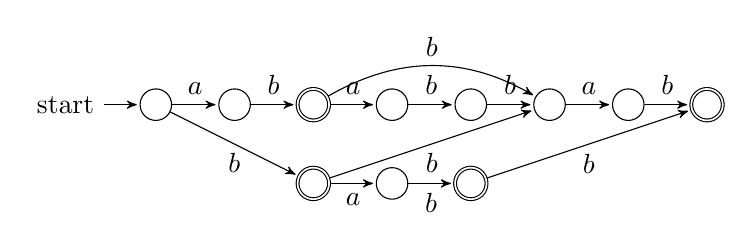
\begin{tikzpicture}[->,>=stealth',shorten >=1pt,auto]
	\tikzstyle{every state} = [circle,draw,minimum size=0.4cm]
	\node[initial,state]	(a)					{};
	\node[state]			(b) [right of=a]	{};
	\node[state,accepting]	(c) [right of=b]	{};
	\node[state]			(d) [right of=c]	{};
	\node[state]			(e) [right of=d]	{};
	\node[state]			(f) [right of=e]	{};
	\node[state]			(g) [right of=f]	{};
	\node[state,accepting]	(h) [right of=g]	{};
	\node[state,accepting]			(i) [below of=c]	{};
	\node[state]			(j) [below of=d]	{};
	\node[state,accepting]	(k) [below of=e]	{};
	\path	(a) edge node {$a$} (b)
				edge [below] node {$b$} (i)
			(b) edge node {$b$} (c)
			(c) edge node {$a$} (d)
				edge [bend left] node {$b$} (f)
			(d) edge node {$b$} (e)
			(e) edge node {$b$} (f)
			(f) edge node {$a$} (g)
			(g) edge node {$b$} (h)
			(i) edge [below] node {$b$} (f)
				edge [below] node {$a$} (j)
			(j) edge [below] node {$b$} (k)
			(k) edge [below] node {$b$} (h);
\end{tikzpicture}

\section{Compressed Suffix automaton}

For $T=ababbab$ construct Compressed Suffix Automaton.

\begin{tikzpicture}[->,>=stealth',shorten >=1pt,auto]
	\tikzstyle{every state} = [circle,draw,minimum size=0.4cm]
	\node[initial,state]	(a)					{};
	\node[state,accepting]	(c) [right of=b]	{};
	\node[state]			(f) [right of=e]	{};
	\node[state,accepting]	(h) [right of=g]	{};
	\node[state,accepting]			(i) [below of=c]	{};
	\node[state,accepting]	(k) [below of=e]	{};
	\path	(a) edge node {$ab$} (c)
				edge node {$b$} (i)
			(c) edge node {$abb$} (f)
				edge [bend left] node {$b$} (f)
			(f) edge node {$ab$} (h)
			(i) edge node {$b$} (f)
				edge node {$ab$} (k)
			(k) edge node {$b$} (h);
\end{tikzpicture}

\clearpage
\section{Suffix Automaton Construction from Suffix Trie}

For $T=ababbab$ construct Suffix Automaton from its Suffix Trie.

States of Suffix Trie are labeled as if it was an automaton.

\tikzstyle{a} = [above]
\tikzstyle{c} = [circle, draw, minimum width=0.4cm]
\tikzstyle{e} = [circle, draw, minimum width=0.4cm, accepting]
\tikzstyle{level 1} = [level distance=1cm, sibling distance=2cm]
\tikzstyle{level 2} = [level distance=1cm, sibling distance=1cm]
\tikzstyle{level 3} = [level distance=1cm, sibling distance=1cm]
\tikzstyle{level 4} = [level distance=1cm, sibling distance=1cm]
\begin{tikzpicture}[grow=right]
	\node[c] {$0$}
	child {
		node[c] {$10$}
		child {
			node[e] {$11$}
			child {
				node[c] {$15$}
				child {
					node[c] {$16$}
					child {
						node[c] {$17$}
						child {
							node[c] {$18$}
							child {
								node[e] {$19$}
								edge from parent
								node[a] {$b$}
							}
							edge from parent
							node[a] {$a$}
						}
						edge from parent
						node[a] {$b$}
					}
					edge from parent
					node[a] {$b$}
				}
				edge from parent
				node[a] {$a$}
			}
			child {
				node[c] {$12$}
				child {
					node[c] {$13$}
					child {
						node[e] {$14$}
						edge from parent
						node[a] {$b$}
					}
					edge from parent
					node[a] {$a$}
				}
				edge from parent
				node[a] {$b$}
			}
			edge from parent
			node[a] {$b$}
		}
		edge from parent
		node[a] {$a$}
	}
	child {
		node[e] {$1$}
		child {
			node[c] {$5$}
			child {
				node[e] {$6$}
				child {
					node[c] {$7$}
					child {
						node[c] {$8$}
						child {
							node[e] {$9$}
							edge from parent
							node[a] {$b$}
						}
						edge from parent
						node[a] {$a$}
					}
					edge from parent
					node[a] {$b$}
				}
				edge from parent
				node[a] {$b$}
			}
			edge from parent
			node[a] {$a$}
		}
		child {
			node[c] {$2$}
			child {
				node[c] {$3$}
				child {
					node[e] {$4$}
					edge from parent
					node[a] {$b$}
				}
				edge from parent
				node[a] {$a$}
			}
			edge from parent
			node[a] {$b$}
		}
		edge from parent
		node[a] {$b$}
	};
\end{tikzpicture}

Transition function is iteratively analyzed. In each iteration the states are put into groups based on their similarity. In the initial interation $g_0$ states are split into two groups: final states and non-final states. The groups are labeled by a first state in the group for convenience. In following in iterations $g_i, i \geq 1$ states are split into groups based on the previsous group and groups to which transions for all symbols of the alphabet lead.

\begin{table}[h]
  \footnotesize
	\begin{tabular}{|c||c|c||c||c|c||c||c|c||c||c|c||c||c|c||c||}
		\hline
		$\delta$ & a & b & $g_0$ & a & b & $g_1$ & a & b & $g_2$ & a & b & $g_3$ & a & b & $g_4$\\ \hline
		0  & 10 & 1  & 0 & 0 & 1 & 0 & 0 & 1 & 0  & 0  & 1  & 0 & 0  & 1  & 0 \\ 
		1  & 5  & 2  & 1 & 0 & 0 & 1 & 0 & 2 & 1  & 0  & 2  & 1 & 0  & 2  & 1 \\
		2  & 3  & -  & 0 & 0 & 0 & 2 & 0 & 2 & 2  & 0  & -  & 2 & 0  & -  & 2 \\
		3  & -  & 4  & 0 & 0 & 1 & 0 & 2 & 1 & 0  & -  & 4  & 3 & -  & 4  & 3 \\
		4  & -  & -  & 1 & 0 & 0 & 1 & 2 & 2 & 4  & -  & -  & 4 & -  & -  & 4 \\
		5  & -  & 6  & 0 & 0 & 1 & 0 & 2 & 1 & 0  & -  & 1  & 5 & -  & 1  & 5 \\
		6  & -  & 7  & 1 & 0 & 0 & 1 & 2 & 2 & 1  & -  & 2  & 6 & -  & 2  & 6 \\
		7  & 8  & -  & 0 & 0 & 0 & 2 & 0 & 2 & 2  & 0  & -  & 2 & 0  & -  & 2 \\
		8  & -  & 9  & 0 & 0 & 1 & 0 & 2 & 1 & 0  & -  & 4  & 3 & -  & 4  & 3 \\
		9  & -  & -  & 1 & 0 & 0 & 1 & 2 & 2 & 4  & -  & -  & 4 & -  & -  & 4 \\
		10 & -  & 11 & 0 & 0 & 1 & 0 & 2 & 1 & 0  & -  & 11 & 10& -  & 11 & 10 \\
		11 & 15 & 12 & 1 & 0 & 0 & 1 & 2 & 2 & 11 & 15 & 2  & 11& 15 & 2  & 11\\
		12 & 13 & -  & 0 & 0 & 0 & 2 & 0 & 2 & 2  & 0  & -  & 2 & 3  & -  & 2 \\
		13 & -  & 14 & 0 & 0 & 1 & 0 & 2 & 1 & 0  & -  & 4  & 3 & -  & 4  & 3 \\
		14 & -  & -  & 1 & 0 & 0 & 1 & 2 & 2 & 4  & -  & -  & 4 & -  & -  & 4 \\
		15 & -  & 16 & 0 & 0 & 0 & 2 & 2 & 2 & 15 & -  & 2  & 15& -  & 2  & 15\\
		16 & -  & 17 & 0 & 0 & 0 & 2 & 2 & 2 & 15 & -  & 15 & 16& -  & 15 & 16\\
		17 & 18 & -  & 0 & 0 & 0 & 2 & 0 & 2 & 2  & 0  & -  & 2 & 3  & -  & 2 \\
		18 & -  & 19 & 0 & 0 & 1 & 0 & 2 & 1 & 0  & -  & 4  & 3 & -  & 4  & 3 \\
		19 & -  & -  & 1 & 0 & 0 & 1 & 2 & 2 & 4  & -  & -  & 4 & -  & -  & 4 \\
		-  & -  & -  & 0 & 0 & 0 & 2 & 2 & 2 & -  & -  & -  & - & -  & -  & - \\
		\hline
	\end{tabular} 
	\caption{Minimization of Suffix Trie for string $T=ababbab$.}
\end{table}

The algorithm ends when either each state is in its own group -- the automaton in already minimal or if two consecutive iterations $g_i$ and $g_{i+1}$ split the states the same way.

States which end up in the same group are equivalent:
\begin{itemize}
	\item $2 \Leftrightarrow 7 \Leftrightarrow 12 \Leftrightarrow 17$,
	\item $3 \Leftrightarrow 8 \Leftrightarrow 13 \Leftrightarrow 18$,
	\item $4 \Leftrightarrow 9 \Leftrightarrow 14 \Leftrightarrow 19$.
\end{itemize}

The equivalent states can be merged together and minimal automaton can be constructed.

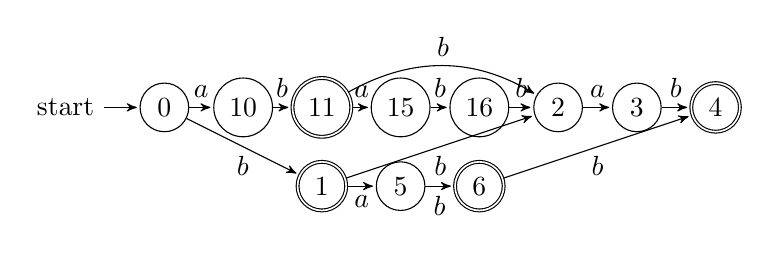
\begin{tikzpicture}[->,>=stealth',shorten >=1pt,auto]
	\tikzstyle{every state} = [circle,draw,minimum size=0.4cm]
	\node[initial,state]	(a)					{$0$};
	\node[state]			(b) [right of=a]	{$10$};
	\node[state,accepting]	(c) [right of=b]	{$11$};
	\node[state]			(d) [right of=c]	{$15$};
	\node[state]			(e) [right of=d]	{$16$};
	\node[state]			(f) [right of=e]	{$2$};
	\node[state]			(g) [right of=f]	{$3$};
	\node[state,accepting]	(h) [right of=g]	{$4$};
	\node[state,accepting]			(i) [below of=c]	{$1$};
	\node[state]			(j) [below of=d]	{$5$};
	\node[state,accepting]	(k) [below of=e]	{$6$};
	\path	(a) edge node {$a$} (b)
				edge [below] node {$b$} (i)
			(b) edge node {$b$} (c)
			(c) edge node {$a$} (d)
				edge [bend left] node {$b$} (f)
			(d) edge node {$b$} (e)
			(e) edge node {$b$} (f)
			(f) edge node {$a$} (g)
			(g) edge node {$b$} (h)
			(i) edge [below] node {$b$} (f)
				edge [below] node {$a$} (j)
			(j) edge [below] node {$b$} (k)
			(k) edge [below] node {$b$} (h);
\end{tikzpicture}

\chapter{Exact string matching}

\section{Naive search}
\begin{itemize}
\item Time complexity: $O(mn)$.
\item Space complexity: $O(1)$.
\end{itemize}

\begin{verbatim}
T = abcabaabaabaacababaabaaba
P = abaabaa

abcabaabaabaacababaabaabaa
aba
 a
  a
   abaabaa                         match on position 3
    a
     ab
      abaabaa                      match on position 6
       a
        ab
         abaab
          a
           ab
            ab
             a
              abaa
               a
                abaabaa            match on position 16
                 a
                  ab
                   abaabaa         match on position 19
                    a
                     ab
                      abaab
                       a
                        ab
\end{verbatim}

\begin{verbatim}
T = aaaaaaaaaaa
P = aaaaa

aaaaaaaaaa
aaaaa            match on position 0
 aaaaa           match on position 1
  aaaaa          match on position 2
   aaaaa         match on position 3
    aaaaa        match on position 4
     aaaaa       match on position 5
      aaaa
       aaa
        aa
         a
\end{verbatim}

%\subsection{Algorithm implementation}
%\cpplistings{tut3/naive}{Naive Search Algorithm.}{{14-36}}

\section{Karp--Robin}

\section{Morris--Pratt}

\begin{itemize}
\item Time complexity: $O(n)$.
\item Space complexity: $O(1)$.
\end{itemize}

\begin{verbatim}
T = abcabaabaabaacababaabaabaa
P = abaabaa

Preprocessing:

Index:    0  1  2  3  4  5  6
String:   a  b  a  a  b  a  a 
Border:   0  0  1  1  2  3  4 
MP:       0  1  1  2  2  3  4  5 

Processing:
abcabaabaabaacababaabaabaa
aba
  a
   abaabaa                   match on position 3
      ????baa                match on position 6
         ????b
            ?b
             a
              abaa
                ?baabaa      match on position 16
                   ????baa   match on position 19
\end{verbatim}

%\subsection{Algorithm implementation}
%\cpplistings{tut3/mp}{Morris-Pratt Algorithm.}

\section{Knuth--Morris--Pratt}

\begin{itemize}
\item Time complexity: $O(n)$.
\item Space complexity: $O(1)$.
\end{itemize}

\begin{verbatim}
T = abcabaabaabaacababaabaabaa
P = abaabaa

Preprocessing:

Index:    0  1  2  3  4  5  6
String:   a  b  a  a  b  a  a
Border:   0  0  1  1  2  3  4
KMP:      0  1  0  2  1  0  2  5

Processing:
abcabaabaabaacababaabaabaa
aba
   abaabaa                   match on position 3
      ????baa                match on position 6
         ????b
             a
              abaa
                ?baabaa      match on position 16
                   ????baa   match on position 19
\end{verbatim}

%\subsection{Algorithm implementation}
%\cpplistings{tut3/kmp}{Knuth--Morris-Pratt Algorithm.}

\section{Boyer--Moore--Horsepool}
\begin{itemize}
\item Time complexity: $O(n)$.
\item Space complexity: $O(1+|\Sigma|)$.
\end{itemize}

\begin{verbatim}
T = abcabaabaabaacababaabaabaa
P = abaabaa

Preprocessing:

Index:    97  98 ???
BCS:       1   2   7 

Processing:
abcabaabaabaacababaabaabaa
..aabaa
 ......a
   abaabaa                   match on position 3
    ......a
      abaabaa                match on position 6
       ......a
              ......a
                abaabaa      match on position 16
                 ......a
                   abaabaa   match on position 19
\end{verbatim}

\begin{verbatim}
T = abcabdaacbabcaaba 
P = bcaab

Preprocessing:

Index:    97  98  99 ???
BCS:       1   4   3   5 

Processing:
abcabdaacbabcaaba
..aab
    ....b
       ..aab
           bcaab    match on position 11
\end{verbatim}

\section{Boyer--Moore--Horsepool--Sunday}

\begin{verbatim}
T = abcabdaacbabcaaba 
P = bcaab

Preprocessing:

Index:    97  98  99 ???
BCS:       2   1   4   6 

Processing:
abcabdaacbabcaaba
..aab
      ....b
       ..aab
           bcaab    match on position 11
\end{verbatim}

\chapter{Other matching methods}

\section{Fisher--Paterson}

For text $T=\texttt{gcatatatgccggata}$ and pattern $P=\texttt{cata}$ perform Fisher--Patterson algorithm.

$T_a=(0,0,1,0,1,0,1,0,0,0,0,0,0,1,0,1)$, $P_a=(0,1,0,1)$\\
$T_c=(0,1,0,0,0,0,0,0,0,1,1,0,0,0,0,0)$, $P_c=(1,0,0,0)$\\
$T_g=(1,0,0,0,0,0,0,0,1,0,0,1,1,0,0,0)$, $P_g=(0,0,0,0)$\\
$T_t=(0,0,0,1,0,1,0,1,0,0,0,0,0,0,1,0)$, $P_t=(0,0,1,0)$\medskip\\
$T_a \times {P_a}^R = (0,0,1,0,2,0,2,0,1,0,0,0,0,1,0,2,0,1,0)$\\
$T_c \times {P_c}^R = (0,0,0,0,1,0,0,0,0,0,0,0,1,1,0,0,0,0,0)$\\
$T_g \times {P_g}^R = (0,0,0,0,0,0,0,0,0,0,0,0,0,0,0,0,0,0,0)$\\
$T_t \times {P_t}^R = (0,0,0,0,1,0,1,0,1,0,0,0,0,0,0,1,0,0,0)$\medskip\\
$R = (0,0,1,0,4,0,3,0,2,0,0,0,1,2,0,3,0,1,0)$

Each position in $R$ represents a number of matched characters when $R$ is aligned with string $T$, $|R| = |T|+ |P| - 1$, so it contains also partial matches.

\section{Rank \& Select}

\clearpage
\section{Wavelet Tree}

\begin{figure}
\tikzstyle{level 1}=[level distance=1.5cm, sibling distance=8cm]
\tikzstyle{level 2}=[level distance=1.5cm, sibling distance=4cm]
\tikzstyle{level 3}=[level distance=1.5cm, sibling distance=4cm]
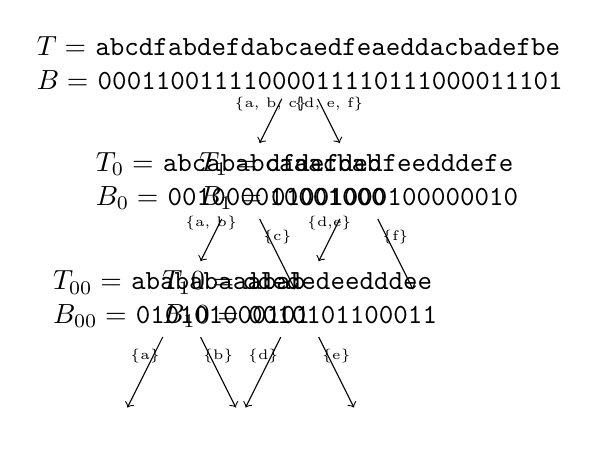
\begin{tikzpicture}[grow=down]
	\node[align=left] {
	 	$T=$ \texttt{abcdfabdefdabcaedfeaeddacbadefbe}\\
		\red$B=$ \texttt{00011001111000011110111000011101}
  }
	child {
		node[align=left] {
			$T_0=$ \texttt{abcababcaaacbab}\\
			\red$B_0=$ \texttt{001000010001000}
		}
		child {
			node[align=left] {
				$T_{00}=$ \texttt{abababaaabab}\\
				\red$B_{00}=$ \texttt{010101000101}
			}
			child {
        node{\texttt{}}
        edge from parent [->] node [midway,above] {\tiny \{a\}}
      }
			child {
        node{\texttt{}}
        edge from parent [->] node [midway,above] {\tiny \{b\}}
      }
      edge from parent [->] node [midway,above] {\tiny \{a, b\}}
		}
		child {
      node{\texttt{}}
      edge from parent [->] node [midway,above] {\tiny \{c\}}
    }
    edge from parent [->] node [midway,above] {\tiny \{a, b, c\}}
	}
	child {
		node[align=left] {
			$T_1=$ \texttt{dfdefdedfeedddefe}\\
			\red$B_1=$ \texttt{01001000100000010}
		}
		child {
			node[align=left]{
				$T_10=$ \texttt{ddededeedddee}\\
				\red$B_10=$ \texttt{0010101100011}
			}
			child {
        node{\texttt{}}
        edge from parent [->] node [midway,above] {\tiny \{d\}}
      }
			child {
        node{\texttt{}}
        edge from parent [->] node [midway,above] {\tiny \{e\}}
      }
      edge from parent [->] node [midway,above] {\tiny \{d,e\}}
		}
		child {
      node{\texttt{}}
      edge from parent [->] node [midway,above] {\tiny \{f\}}
    }
    edge from parent [->] node [midway,above] {\tiny \{d, e, f\}}
	};
\end{tikzpicture}
\caption{Wavelet tree for string $T$=abcdfabdefdabcaedfeaeddacbadefbe.}
\end{figure}

$\mathrm{rank}_T(\texttt{b}, 10) = \mathrm{rank}_{B_{00}}(1, \mathrm{rank}_{B_0}(0, \mathrm{rank}_B(0, 10)))$\\
$\mathrm{select}_T(\texttt{d}, 5) = \mathrm{select}_B(1, \mathrm{select}_{B_1}(0, \mathrm{select}_{B_{10}}(0, 5)))$

Support rank, select and symbol on posstion queris.

\section{Compressed Suffix Array}

\chapter{FM--index}

Create FM--index for text $T=\texttt{abracadabra}$ and perform search algorithm with pattern $P = \texttt{bdabra}$.

\begin{tabular}{c|ccccccccccc}
 	$i$		&1 			&2 			&3 			&4 			&5 			&6 			&7 			&8 			&9 			&10 		&11 \\\hline
	$T[i]$			&\texttt{a}	&\texttt{b}	&\texttt{r}	&\texttt{a}	&\texttt{c}	&\texttt{a}	&\texttt{d}	&\texttt{a}	&\texttt{b}	&\texttt{r}	&\texttt{a}	\\\hline
	$SA[i]$		&11			&8			&1			&4			&6			&9			&2			&5			&7			&10			&3			\\\hline
	$SA[i]-1$	&10			&7			&11			&3			&5			&8			&1			&4			&6			&9			&2			\\\hline
	$L=T[SA[i]]$	&\texttt{r}	&\texttt{d}	&\texttt{a}	&\texttt{r}	&\texttt{c}	&\texttt{a}	&\texttt{a}	&\texttt{a}	&\texttt{a}	&\texttt{b}	&\texttt{b}	\\\hline
	$F=T[SA[i]-1]$	&\texttt{a}	&\texttt{a}	&\texttt{a}	&\texttt{a}	&\texttt{a}	&\texttt{b}	&\texttt{b}	&\texttt{c}	&\texttt{d}	&\texttt{r}	&\texttt{r}	\\\hline
\end{tabular}
\begin{tabular}{|ll}
11:	&\texttt{{\red{a}}abracadab{\blue{r}}}\\
8:	&\texttt{{\red{a}}braabraca{\blue{d}}}\\
1:	&\texttt{{\red{a}}bracadabr{\blue{a}}}\\
4:	&\texttt{{\red{a}}cadabraab{\blue{r}}}\\
6:	&\texttt{{\red{a}}dabraabra{\blue{c}}}\\
9:	&\texttt{{\red{b}}raabracad{\blue{a}}}\\
2:	&\texttt{{\red{b}}racadabra{\blue{a}}}\\
5:	&\texttt{{\red{c}}adabraabr{\blue{a}}}\\
7:	&\texttt{{\red{d}}abraabrac{\blue{a}}}\\
10:	&\texttt{{\red{r}}aabracada{\blue{b}}}\\
3:	&\texttt{{\red{r}}acadabraa{\blue{b}}}\\
\end{tabular}

\begin{enumerate}
\item[0.] \begin{itemize}
	\item $L = \texttt{rdarcaaaabb}$
	\item $P = \texttt{bdabra}$
	\item
		\begin{tabular}{c|ccccc}
		$c$	&\texttt{a}	&\texttt{b}	&\texttt{c}	&\texttt{d}	&\texttt{r}	\\\hline
		$C$	&0			&5			&7			&8			&9			\\
		\end{tabular}
	\item $sp_i = C[c] + Occ(L, c, sp_{i-1}-1)+1$
	\item $ep_i = C[c] + Occ(L, c, ep_{i-1})$
	\item $occ_x = ep - sp + 1$
	\item $sp_0 = 1$, $ep_0 = \left| L \right| = 11$
	\end{itemize}
\end{enumerate}
%\begin{multicols}{2}
\begin{enumerate}
\item \begin{itemize}
	\item $P=\texttt{bdabr{\red{a}}}$
	\item $sp_1 = 0+0+1 = 1$
	\item $ep_1 = 0+5 = 5$
	\item $occ_{a} = 5-1+1 = 5$
	\end{itemize}
\item \begin{itemize}
	\item $P=\texttt{bdab{\red{r}}a}$
	\item $sp_2 = 9+0+1 = 10$
	\item $ep_2 = 9+2 = 11$
	\item $occ_{ra} = 11-10+1 = 2$
	\end{itemize}
\item \begin{itemize}
	\item $P=\texttt{bda{\red{b}}ra}$
	\item $sp_3 = 5+0+1 = 6$
	\item $ep_3 = 5+2 = 7$
	\item $occ_{bra} = 7-6+1 = 2$
	\end{itemize}
\item \begin{itemize}
	\item $P=\texttt{bd{\red{a}}bra}$
	\item $sp_4 = 0+1+1 = 2$
	\item $ep_4 = 0+3 = 3$
	\item $occ_{abra} = 3-2+1 = 2$
	\end{itemize}
\item \begin{itemize}
	\item $P=\texttt{b{\red{d}}abra}$
	\item $sp_5 = 8+0+1 = 9$
	\item $ep_5 = 8+1 = 9$
	\item $occ_{dabra} = 9-9+1 = 1$
	\end{itemize}
\item \begin{itemize}
	\item $P=\texttt{{\red{b}}dabra}$
	\item $sp_2 = 5+0+1 = 6$
	\item $ep_2 = 5+0 = 5$
	\item $occ_{bdabra} = 5-6+1 = 0$
	\end{itemize}
\end{enumerate}
%\end{multicols}

\chapter{Approximate string matching}

\section{Edit (Levensthein) distance}

\begin{equation*}
  \qquad\operatorname{d}_{t,p}(i,j) =
  \begin{cases}
    \max(i,j) & \text{ if } \min(i,j)=0, \\
    \min
      \begin{cases}
        \operatorname{d}_{t,p}(i-1,j) + 1 \\
        \operatorname{d}_{t,p}(i,j-1) + 1 \\
        \operatorname{d}_{t,p}(i-1,j-1) + 1_{(t_i \neq p_j)}
      \end{cases} & \text{ otherwise.}
  \end{cases}
\end{equation*}

\begin{table}
  \begin{center}
    \begin{tabular}{c|ccccccc}
                  &\texttt{-}		&\texttt{a}		&\texttt{g}		&\texttt{t}		&\texttt{c}		&\texttt{a}		&\texttt{g}\\
      \hline
      \texttt{-}	&\tm{l10}0\tm{r10}  &\tm{l11}1\tm{r11}	&\tm{l12}2\tm{r12}  &\tm{l13}3\tm{r13}  &\tm{l14}4\tm{r14}	&\tm{l15}5\tm{r15}	&\tm{l16}6\tm{r16}\\[2px]
      \texttt{g}	&\tm{l20}1\tm{r20}	&\tm{l21}1\tm{r21}	&\tm{l22}1\tm{r22}	&\tm{l23}2\tm{r23}	&\tm{l24}3\tm{r24}	&\tm{l25}4\tm{r25}	&\tm{l26}5\tm{r26}\\[2px]
      \texttt{a}	&\tm{l30}2\tm{r30}	&\tm{l31}1\tm{r31}	&\tm{l32}2\tm{r32}	&\tm{l33}2\tm{r33}	&\tm{l34}3\tm{r34}	&\tm{l35}3\tm{r35}	&\tm{l36}4\tm{r36}\\[2px]
      \texttt{t}	&\tm{l40}3\tm{r40}	&\tm{l41}2\tm{r41}	&\tm{l42}2\tm{r42}	&\tm{l43}2\tm{r43}	&\tm{l44}3\tm{r44}	&\tm{l45}4\tm{r45}	&\tm{l46}4\tm{r46}\\[2px]
      \texttt{c}	&\tm{l50}4\tm{r50}	&\tm{l51}3\tm{r51}	&\tm{l52}3\tm{r52}	&\tm{l53}3\tm{r53}	&\tm{l54}2\tm{r54}	&\tm{l55}3\tm{r55}	&\tm{l56}4\tm{r56}\\[2px]
      \texttt{a}	&\tm{l60}5\tm{r60}  &\tm{l61}4\tm{r61}	&\tm{l62}4\tm{r62}	&\tm{l63}4\tm{r63}	&\tm{l64}3\tm{r64}	&\tm{l65}2\tm{r65}	&\tm{l66}3\tm{r66}\\[2px]
    \end{tabular}
%    \begin{tikzpicture}
%      [
%        remember picture, 
%        overlay, 
%        -latex,
%        shorten >=2pt,
%        shorten <=2pt
%      ]
%      \draw[green] ([yshift=0.5ex]{pic cs:l11}) -- ([yshift=0.5ex]{pic cs:r10});
%      \draw[blue] ([yshift=0.5ex]{pic cs:l12}) -- ([yshift=0.5ex]{pic cs:r11});
%      \draw[blue] ([yshift=0.5ex]{pic cs:l13}) -- ([yshift=0.5ex]{pic cs:r12});
%      \draw[blue] ([yshift=0.5ex]{pic cs:l14}) -- ([yshift=0.5ex]{pic cs:r13});
%      \draw[blue] ([yshift=0.5ex]{pic cs:l15}) -- ([yshift=0.5ex]{pic cs:r14});
%      \draw[blue] ([yshift=0.5ex]{pic cs:l16}) -- ([yshift=0.5ex]{pic cs:r15});
%      
%      \draw[green] ([yshift=1.0ex,xshift=-0.5ex]{pic cs:r20}) -- ([xshift=-0.5ex]{pic cs:r10});
%      \draw[blue] ([yshift=1.0ex,xshift=-0.5ex]{pic cs:r30}) -- ([xshift=-0.5ex]{pic cs:r20});
%      \draw[blue] ([yshift=1.0ex,xshift=-0.5ex]{pic cs:r40}) -- ([xshift=-0.5ex]{pic cs:r30});
%      \draw[blue] ([yshift=1.0ex,xshift=-0.5ex]{pic cs:r50}) -- ([xshift=-0.5ex]{pic cs:r40});
%      \draw[blue] ([yshift=1.0ex,xshift=-0.5ex]{pic cs:r60}) -- ([xshift=-0.5ex]{pic cs:r50});
%
%      \draw[green] ([yshift=1.0ex]{pic cs:l21}) -- ([yshift=0.0ex]{pic cs:r10});
%      \draw[green] ([yshift=1.0ex]{pic cs:l22}) -- ([yshift=0.0ex]{pic cs:r11});
%      \draw[blue] ([yshift=0.5ex]{pic cs:l23}) -- ([yshift=0.5ex]{pic cs:r22});
%      \draw[blue] ([yshift=0.5ex]{pic cs:l24}) -- ([yshift=0.5ex]{pic cs:r23});
%      \draw[blue] ([yshift=0.5ex]{pic cs:l25}) -- ([yshift=0.5ex]{pic cs:r24});
%      \draw[blue] ([yshift=1.0ex]{pic cs:l26}) -- ([yshift=0.0ex]{pic cs:r15});
%
%      \draw[green] ([yshift=1.0ex]{pic cs:l31}) -- ([yshift=0.0ex]{pic cs:r20});
%      \draw[green] ([yshift=1.0ex]{pic cs:l32}) -- ([yshift=0.0ex]{pic cs:r21});
%      \draw[blue] ([yshift=1.0ex]{pic cs:l33}) -- ([yshift=0.0ex]{pic cs:r22});
%      \draw[blue] ([yshift=1.0ex]{pic cs:l34}) -- ([yshift=0.0ex]{pic cs:r23});
%      \draw[blue] ([yshift=1.0ex]{pic cs:l35}) -- ([yshift=0.0ex]{pic cs:r24});
%      \draw[blue] ([yshift=0.5ex]{pic cs:l36}) -- ([yshift=0.5ex]{pic cs:r35});
%
%      \draw[blue] ([yshift=1.0ex,xshift=-0.5ex]{pic cs:r41}) -- ([xshift=-0.5ex]{pic cs:r31});
%      \draw[blue] ([yshift=1.0ex]{pic cs:l42}) -- ([yshift=0.0ex]{pic cs:r31});
%      \draw[green] ([yshift=1.0ex]{pic cs:l43}) -- ([yshift=0.0ex]{pic cs:r32});
%      \draw[blue] ([yshift=1.0ex]{pic cs:l44}) -- ([yshift=0.0ex]{pic cs:r33});
%      \draw[blue] ([yshift=1.0ex]{pic cs:l45}) -- ([yshift=0.0ex]{pic cs:r34});
%      \draw[blue] ([yshift=1.0ex]{pic cs:l46}) -- ([yshift=0.0ex]{pic cs:r35});
%
%      \draw[blue] ([yshift=1.0ex,xshift=-0.5ex]{pic cs:r51}) -- ([xshift=-0.5ex]{pic cs:r41});
%      \draw[blue] ([yshift=1.0ex]{pic cs:l52}) -- ([yshift=0.0ex]{pic cs:r41});
%      \draw[blue] ([yshift=1.0ex]{pic cs:l53}) -- ([yshift=0.0ex]{pic cs:r42});
%      \draw[green] ([yshift=1.0ex]{pic cs:l54}) -- ([yshift=0.0ex]{pic cs:r43});
%      \draw[blue] ([yshift=0.5ex]{pic cs:l55}) -- ([yshift=0.5ex]{pic cs:r54});
%      \draw[blue] ([yshift=0.5ex]{pic cs:l56}) -- ([yshift=0.5ex]{pic cs:r55});
%      
%      \draw[blue] ([yshift=1.0ex]{pic cs:l61}) -- ([yshift=0.0ex]{pic cs:r50});
%      \draw[blue] ([yshift=1.0ex]{pic cs:l62}) -- ([yshift=0.0ex]{pic cs:r51});
%      \draw[blue] ([yshift=1.0ex]{pic cs:l63}) -- ([yshift=0.0ex]{pic cs:r52});
%      \draw[blue] ([yshift=1.0ex,xshift=-0.5ex]{pic cs:r64}) -- ([xshift=-0.5ex]{pic cs:r54});
%      \draw[green] ([yshift=1.0ex]{pic cs:l65}) -- ([yshift=0.0ex]{pic cs:r54});
%      \draw[green] ([yshift=0.5ex]{pic cs:l66}) -- ([yshift=0.5ex]{pic cs:r65});
%      
%      \draw[green] ([yshift=1.0ex,xshift=-0.5ex]{pic cs:r32}) -- ([xshift=-0.5ex]{pic cs:r22});
%      \draw[green] ([yshift=0.5ex]{pic cs:l32}) -- ([yshift=0.5ex]{pic cs:r31});
%    \end{tikzpicture}
  \end{center}
  \caption{Edit distance between $t=\texttt{agtcag}$ a $p=\texttt{gatca}$.}
\end{table}

\clearpage
\section{Weighted edit distance}

\begin{equation*}
  \qquad\operatorname{d}_{t,p}(i,j) =
  \begin{cases}
    0 & \text{ if } i=0 \land j = 0,\\
    {d}_{t,p}(i-1,0) + D(t_i) & \text{ if } j=0 \land i > 0, \\
    {d}_{t,p}(0,j-1) + I(p_j) & \text{ if } i=0 \land j > 0, \\
    \min
      \begin{cases}
        \operatorname{d}_{t,p}(i-1,j) + D(t_i) \\
        \operatorname{d}_{t,p}(i,j-1) + I(p_j) \\
        \operatorname{d}_{t,p}(i-1,j-1) + R(p_j,t_i)_{(t_i \neq p_j)}
      \end{cases} & \text{ otherwise.}
  \end{cases}
\end{equation*}

\begin{table}
  \begin{center}
    \begin{tabular}{cc}
      \begin{tabular}[t]{c|cccc}
        R   &\texttt{a} &\texttt{g} &\texttt{c} &\texttt{t}\\\hline
        \texttt{a}  &-   &2   &3   &4\\
        \texttt{g}  &2   &-   &6   &2\\
        \texttt{c}  &2   &5   &-   &1\\
        \texttt{t}  &5   &2   &1   &-\\\hline
        I   &5 &2 &4 &3\\
        D   &2 &5 &3 &4\\
      \end{tabular}
      \quad
      \begin{tabular}[t]{c|ccccccc}
        DP          &\texttt{-}		&\texttt{a}		&\texttt{g}		&\texttt{t}		&\texttt{c}		&\texttt{a}		&\texttt{g}\\
        \hline
        \texttt{-}	&\tm{l10} 0\tm{r10}  &\tm{l11} 2\tm{r11}	&\tm{l12} 7\tm{r12} &\tm{l13}11\tm{r13} &\tm{l14}14\tm{r14}	&\tm{l15}16\tm{r15}	&\tm{l16}21\tm{r16}\\[2px]
        \texttt{g}	&\tm{l20} 2\tm{r20}	 &\tm{l21} 2\tm{r21}	&\tm{l22} 2\tm{r22}	&\tm{l23} 6\tm{r23}	&\tm{l24} 9\tm{r24}	&\tm{l25}11\tm{r25}	&\tm{l26}16\tm{r26}\\[2px]
        \texttt{a}	&\tm{l30} 7\tm{r30}	 &\tm{l31} 2\tm{r31}	&\tm{l32} 4\tm{r32}	&\tm{l33} 6\tm{r33}	&\tm{l34} 9\tm{r34}	&\tm{l35} 9\tm{r35}	&\tm{l36}13\tm{r36}\\[2px]
        \texttt{t}	&\tm{l40}10\tm{r40}	 &\tm{l41} 5\tm{r41}	&\tm{l42} 4\tm{r42}	&\tm{l43} 4\tm{r43}	&\tm{l44} 7\tm{r44}	&\tm{l45} 9\tm{r45}	&\tm{l46}11\tm{r46}\\[2px]
        \texttt{c}	&\tm{l50}14\tm{r50}	 &\tm{l51}9\tm{r51}	&\tm{l52} 8\tm{r52}	&\tm{l53} 5\tm{r53}	&\tm{l54} 4\tm{r54}	&\tm{l55} 6\tm{r55}	&\tm{l56}11\tm{r56}\\[2px]
        \texttt{a}	&\tm{l60}19\tm{r60}  &\tm{l61}14\tm{r61}	&\tm{l62}11\tm{r62}	&\tm{l63} 10\tm{r63}	&\tm{l64} 8\tm{r64}	&\tm{l65} 4\tm{r65}	&\tm{l66}8\tm{r66}\\[2px]
      \end{tabular}
    \end{tabular}
  \end{center}
  \caption{Weighted edit distance between $t=\texttt{agtcag}$ a $p=\texttt{gatca}$.}
\end{table}

\clearpage
\section{Needleman--Wunsch}

\begin{equation*}
  \qquad\operatorname{d}_{t,p}(i,j) =
  \begin{cases}
    0 & \text{ if } i=0 \land j = 0,\\
    i \cdot c & \text{ if } j=0 \land i > 0, \\
    j \cdot c & \text{ if } i=0 \land j > 0, \\
    \max
      \begin{cases}
        \operatorname{d}_{t,p}(i-1,j) + c \\
        \operatorname{d}_{t,p}(i,j-1) + c \\
        \operatorname{d}_{t,p}(i-1,j-1) + S(p_j,t_i)
      \end{cases} & \text{ otherwise.}
  \end{cases}
\end{equation*}


\begin{table}
  \begin{center}
    \begin{tabular}{cc}
      \begin{tabular}[t]{c|cccc}
        S   &\texttt{a} &\texttt{g} &\texttt{c} &\texttt{t}\\\hline
        \texttt{a}  &10   &-1   &-3   &-4\\
        \texttt{g}  &-1   &7    &-5   &-3\\
        \texttt{c}  &-3   &-5   &9    &0\\
        \texttt{t}  &-4   &-3   &0    &8\\\hline
        c  & -5 \\
      \end{tabular}
      \quad
      \begin{tabular}[t]{c|ccccccc}
        DP          &\texttt{-}		&\texttt{a}		&\texttt{g}		&\texttt{t}		&\texttt{c}		&\texttt{a}		&\texttt{g}\\
        \hline
        \texttt{-}	&\tm{l10}  0\tm{r10}  &\tm{l11} -5\tm{r11}	&\tm{l12}-10\tm{r12}    &\tm{l13}-15\tm{r13}    &\tm{l14}-20\tm{r14}	&\tm{l15}-25\tm{r15}	&\tm{l16}-30\tm{r16}\\[2px]
        \texttt{g}	&\tm{l20} -5\tm{r20}  &\tm{l21} -1\tm{r21}	&\tm{l22}  2\tm{r22}	&\tm{l23} -3\tm{r23}	&\tm{l24} -8\tm{r24}	&\tm{l25}-13\tm{r25}	&\tm{l26}-18\tm{r26}\\[2px]
        \texttt{a}	&\tm{l30}-10\tm{r30}  &\tm{l31}  5\tm{r31}	&\tm{l32}  0\tm{r32}	&\tm{l33} -2\tm{r33}	&\tm{l34} -6\tm{r34}	&\tm{l35}  2\tm{r35}	&\tm{l36} -3\tm{r36}\\[2px]
        \texttt{t}	&\tm{l40}-15\tm{r40}  &\tm{l41}  0\tm{r41}	&\tm{l42}  2\tm{r42}	&\tm{l43}  8\tm{r43}	&\tm{l44}  3\tm{r44}	&\tm{l45} -2\tm{r45}	&\tm{l46} -1\tm{r46}\\[2px]
        \texttt{c}	&\tm{l50}-20\tm{r50}  &\tm{l51} -5\tm{r51}	&\tm{l52} -3\tm{r52}	&\tm{l53}  3\tm{r53}	&\tm{l54}  17\tm{r54}	&\tm{l55} 12\tm{r55}	&\tm{l56} 7\tm{r56}\\[2px]
        \texttt{a}	&\tm{l60}-25\tm{r60}  &\tm{l61}-10\tm{r61}	&\tm{l62} -6\tm{r62}	&\tm{l63} -2\tm{r63}	&\tm{l64} 12\tm{r64}	&\tm{l65}  27\tm{r65}	&\tm{l66}  22\tm{r66}\\[2px]
      \end{tabular}
    \end{tabular}
  \end{center}
  \caption{Needleman--Wunsch price of alignment between $t=\texttt{agtcag}$ a $p=\texttt{gatca}$.}
\end{table}

\clearpage
\section{Algorithm implementations}
\cpplistings{tut6/levensthein}{Implementation of Levenshtein distance algorithm.}{{17-44}}
  \clistings{tut6/distance}{Implementation of Levenshein distance algorithm with backtracking.}{{23-61}}
\cpplistings{tut6/wed}{Implementation of Weighted edit distance algorithm.}{{89-134}}
\cpplistings{tut6/nw}{Implementation of Needleman--Wunsch algorithm.}{{73-106}}


\clearpage
\chapter*{Conslusion}

\newthought{This materials} are are still work in progress.

I thank you very much for reading them, using them and helping me improve them by your input.

To be continued\ldots

\raggedleft \emph{Ing. Radomír Polách}

%\chapter{The Design of Tufte's Books}
%\label{ch:tufte-design}
%
%\newthought{The pages} of a book are usually divided into three major
%sections: the front matter (also called preliminary matter or prelim), the
%main matter (the core text of the book), and the back matter (or end
%matter).
%
%\newthought{The front matter} of a book refers to all of the material that
%comes before the main text.  The following table from shows a list of
%material that appears in the front matter of \VDQI, \EI, \VE, and \BE
%along with its page number.  Page numbers that appear in parentheses refer
%to folios that do not have a printed page number (but they are still
%counted in the page number sequence).
%
%\bigskip
%\begin{minipage}{\textwidth}
%\begin{center}
%\begin{tabular}{lcccc}
%\toprule
% & \multicolumn{4}{c}{Books} \\
%%\cmidrule(l){2-5} 
%Page content & \vdqi & \ei & \ve & \be \\
%\midrule
%Blank half title page & \hangp{1} & \hangp{1} & \hangp{1} & \hangp{1} \\
%Frontispiece\footnotemark{}
%  & \hangp{2} & \hangp{2} & \hangp{2} & \hangp{2} \\
%Full title page & \hangp{3} & \hangp{3} & \hangp{3} & \hangp{3} \\
%Copyright page & \hangp{4} & \hangp{4} & \hangp{4} & \hangp{4} \\
%Contents & \hangp{5} & \hangp{5} & \hangp{5} & \hangp{5} \\
%%Blank & -- & \hangp{6} & \hangp{6} & \hangp{6} \\
%Dedication & \hangp{6} & \hangp{7} & \hangp{7} & 7 \\
%%Blank & -- & \hangp{8} & -- & \hangp{8} \\
%Epigraph & -- & -- & \hangp{8} & -- \\
%Introduction & \hangp{7} & \hangp{9} & \hangp{9} & 9 \\
%\bottomrule
%\end{tabular}
%\end{center}
%\end{minipage}
%\vspace{-7\baselineskip}\footnotetext{The contents of this page vary from book to book.  In
%  \vdqi this page is blank; in \ei and \ve this page holds a frontispiece;
%  and in \be this page contains three epigraphs.}
%\vspace{7\baselineskip}
%
%\bigskip
%The design of the front matter in Tufte's books varies slightly from the
%traditional design of front matter.  First, the pages in front matter are
%traditionally numbered with lowercase roman numerals (\eg, i, ii, iii,
%iv,~\ldots).  Second, the front matter page numbering sequence is usually
%separate from the main matter page numbering.  That is, the page numbers
%restart at 1 when the main matter begins.  In contrast, Tufte has
%enumerated his pages with arabic numerals that share the same page counting
%sequence as the main matter.  
%
%There are also some variations in design across Tufte's four books.  The
%page opposite the full title page (labeled ``frontispiece'' in the above
%table) has different content in each of the books.  In \VDQI, this page is
%blank; in \EI and \VE, this page holds a frontispiece; and in \BE, this
%page contains three epigraphs.
%
%The dedication appears on page~6 in \vdqi (opposite the introduction), and
%is placed on its own spread in the other books.  In \ve, an epigraph shares
%the spread with the opening page of the introduction.
%
%None of the page numbers (folios) of the front matter are expressed except in
%\be, where the folios start to appear on the dedication page.
%
%\newthought{The full title page} of each of the books varies slightly in
%design.  In all the books, the author's name appears at the top of the
%page, the title it set just above the center line, and the publisher is
%printed along the bottom margin.  Some of the differences are outlined in
%the following table.
%
%\bigskip
%\begin{center}
%\footnotesize
%\begin{tabular}{lllll}
%\toprule
%Feature & \vdqi & \ei & \ve & \be \\
%\midrule
%Author & & & & \\
%\quad Typeface & serif   & serif   & serif   & sans serif \\
%\quad Style    & italics & italics & italics & upright, caps \\
%\quad Size     & 24 pt   & 20 pt   & 20 pt   & 20 pt \\
%\addlinespace
%Title & & & & \\
%\quad Typeface & serif   & serif   & serif   & sans serif \\
%\quad Style    & upright & italics & upright & upright, caps \\
%\quad Size     & 36 pt   & 48 pt   & 48 pt   & 36 pt \\
%\addlinespace
%Subtitle & & & & \\
%\quad Typeface & \na     & \na     & serif   & \na \\
%\quad Style    & \na     & \na     & upright & \na \\
%\quad Size     & \na     & \na     & 20 pt   & \na \\
%\addlinespace
%Edition & & & & \\
%\quad Typeface & sans serif    & \na  & \na  & \na \\
%\quad Style    & upright, caps & \na  & \na  & \na \\
%\quad Size     & 14 pt         & \na  & \na  & \na \\
%\addlinespace
%Publisher & & & & \\
%\quad Typeface & serif   & serif   & serif   & sans serif \\
%\quad Style    & italics & italics & italics & upright, caps \\
%\quad Size     & 14 pt   & 14 pt   & 14 pt   & 14 pt \\
%\bottomrule
%\end{tabular}
%\end{center}
%
%\begin{figure*}[p]
%\fbox{\includegraphics[width=0.45\linewidth]{graphics/vdqi-title.pdf}}
%\hfill
%\fbox{\includegraphics[width=0.45\linewidth]{graphics/ei-title.pdf}}
%\\\vspace{\baselineskip}
%\fbox{\includegraphics[width=0.45\linewidth]{graphics/ve-title.pdf}}
%\hfill
%\fbox{\includegraphics[width=0.45\linewidth]{graphics/be-title.pdf}}
%\end{figure*}
%
%\newthought{The tables of contents} in Tufte's books give us our first
%glimpse of the structure of the main matter.  \VDQI is split into two
%parts, each containing some number of chapters.  His other three books only
%contain chapters---they're not broken into parts.
%
%\begin{figure*}[p]\index{table of contents}
%\fbox{\includegraphics[width=0.45\linewidth]{graphics/vdqi-contents.pdf}}
%\hfill
%\fbox{\includegraphics[width=0.45\linewidth]{graphics/ei-contents.pdf}}
%\\\vspace{\baselineskip}
%\fbox{\includegraphics[width=0.45\linewidth]{graphics/ve-contents.pdf}}
%\hfill
%\fbox{\includegraphics[width=0.45\linewidth]{graphics/be-contents.pdf}}
%\end{figure*}
%
%
%\section{Typefaces}\label{sec:typefaces1}\index{typefaces}
%\index{fonts|see{typefaces}}
%
%Tufte's books primarily use two typefaces: Bembo and Gill Sans.  Bembo is used
%for the headings and body text, while Gill Sans is used for the title page and
%opening epigraphs in \BE.
%
%Since neither Bembo nor Gill Sans are available in default \LaTeX{}
%installations, the \TL document classes default to using Palatino and
%Helvetica, respectively.  In addition, the Bera Mono typeface is used for
%\texttt{monospaced} type.
%
%The following font sizes are defined by the \TL classes:
%
%\begin{table}[h]\index{typefaces!sizes}
%  \footnotesize%
%  \begin{center}
%    \begin{tabular}{lccl}
%      \toprule
%      \LaTeX{} size & Font size & Leading & Used for \\
%      \midrule
%      \verb+\tiny+         &  5 &  6 & sidenote numbers \\
%      \verb+\scriptsize+   &  7 &  8 & \na \\
%      \verb+\footnotesize+ &  8 & 10 & sidenotes, captions \\
%      \verb+\small+        &  9 & 12 & quote, quotation, and verse environments \\
%      \verb+\normalsize+   & 10 & 14 & body text \\
%      \verb+\large+        & 11 & 15 & \textsc{b}-heads \\
%      \verb+\Large+        & 12 & 16 & \textsc{a}-heads, \textsc{toc} entries, author, date \\
%      \verb+\LARGE+        & 14 & 18 & handout title \\
%      \verb+\huge+         & 20 & 30 & chapter heads \\
%      \verb+\Huge+         & 24 & 36 & part titles \\
%      \bottomrule
%    \end{tabular}
%  \end{center}
%  \caption{A list of \LaTeX{} font sizes as defined by the \TL document classes.}
%  \label{tab:font-sizes}
%\end{table}
%
%\section{Headings}\label{sec:headings1}\index{headings}
%
%Tufte's books include the following heading levels: parts,
%chapters,\sidenote{Parts and chapters are defined for the \texttt{tufte-book}
%class only.}  sections, subsections, and paragraphs.  Not defined by default
%are: sub-subsections and subparagraphs.
%
%\begin{table}[h]
%  \begin{center}
%    \footnotesize%
%    \begin{tabular}{lcr}
%      \toprule
%      Heading & Style & Size \\
%      \midrule
%      Part & roman & \measure{24}{36}{40} \\
%      Chapter & italic & \measure{20}{30}{40} \\
%      Section & italic & \measure{12}{16}{26} \\
%      Subsection & italic & \measure{11}{15}{26} \\
%      Paragraph & italic & 10/14 \\
%      \bottomrule
%    \end{tabular}
%  \end{center}
%  \caption{Heading styles used in \BE.}
%  \label{tab:heading-styles}
%\end{table}
%
%\paragraph{Paragraph} Paragraph headings (as shown here) are introduced by
%italicized text and separated from the main paragraph by a bit of space.
%
%\section{Environments}
%
%The following characteristics define the various environments:
%
%
%\begin{table}[h]
%  \begin{center}
%    \footnotesize%
%    \begin{tabular}{lcl}
%      \toprule
%      Environment & Font size & Notes \\
%      \midrule
%      Body text & \measure{10}{14}{26} & \\
%      Block quote & \measure{9}{12}{24} & Block indent (left and right) by \unit[1]{pc} \\
%      Sidenotes & \measure{8}{10}{12} & Sidenote number is set inline, followed by word space \\
%      Captions & \measure{8}{10}{12} &  \\
%      \bottomrule
%    \end{tabular}
%  \end{center}
%  \caption{Environment styles used in \BE.}
%  \label{tab:environment-styles}
%\end{table}
%
%
%\chapter[On the Use of the tufte-book Document Class]{On the Use of the \texttt{tufte-book} Document Class}
%\label{ch:tufte-book}
%
%The \TL document classes define a style similar to the
%style Edward Tufte uses in his books and handouts.  Tufte's style is known
%for its extensive use of sidenotes, tight integration of graphics with
%text, and well-set typography.  This document aims to be at once a
%demonstration of the features of the \TL document classes
%and a style guide to their use.
%
%\section{Page Layout}\label{sec:page-layout}
%\subsection{Headings}\label{sec:headings}\index{headings}
%This style provides \textsc{a}- and \textsc{b}-heads (that is,
%\Verb|\section| and \Verb|\subsection|), demonstrated above.
%
%If you need more than two levels of section headings, you'll have to define
%them yourself at the moment; there are no pre-defined styles for anything below
%a \Verb|\subsection|.  As Bringhurst points out in \textit{The Elements of
%Typographic Style},\cite{Bringhurst2005} you should ``use as many levels of
%headings as you need: no more, and no fewer.''
%
%The \TL classes will emit an error if you try to use
%\linebreak\Verb|\subsubsection| and smaller headings.
%
%% let's start a new thought -- a new section
%\newthought{In his later books},\cite{Tufte2006} Tufte
%starts each section with a bit of vertical space, a non-indented paragraph,
%and sets the first few words of the sentence in \textsc{small caps}.  To
%accomplish this using this style, use the \doccmddef{newthought} command:
%\begin{docspec}
%  \doccmd{newthought}\{In his later books\}, Tufte starts\ldots
%\end{docspec}
%
%
%\section{Sidenotes}\label{sec:sidenotes}
%One of the most prominent and distinctive features of this style is the
%extensive use of sidenotes.  There is a wide margin to provide ample room
%for sidenotes and small figures.  Any \doccmd{footnote}s will automatically
%be converted to sidenotes.\footnote{This is a sidenote that was entered
%using the \texttt{\textbackslash footnote} command.}  If you'd like to place ancillary
%information in the margin without the sidenote mark (the superscript
%number), you can use the \doccmd{marginnote} command.\marginnote{This is a
%margin note.  Notice that there isn't a number preceding the note, and
%there is no number in the main text where this note was written.}
%
%The specification of the \doccmddef{sidenote} command is:
%\begin{docspec}
%  \doccmd{sidenote}[\docopt{number}][\docopt{offset}]\{\docarg{Sidenote text.}\}
%\end{docspec}
%
%Both the \docopt{number} and \docopt{offset} arguments are optional.  If you
%provide a \docopt{number} argument, then that number will be used as the
%sidenote number.  It will change of the number of the current sidenote only and
%will not affect the numbering sequence of subsequent sidenotes.
%
%Sometimes a sidenote may run over the top of other text or graphics in the
%margin space.  If this happens, you can adjust the vertical position of the
%sidenote by providing a dimension in the \docopt{offset} argument.  Some
%examples of valid dimensions are:
%\begin{docspec}
%  \ttfamily 1.0in \qquad 2.54cm \qquad 254mm \qquad 6\Verb|\baselineskip|
%\end{docspec}
%If the dimension is positive it will push the sidenote down the page; if the
%dimension is negative, it will move the sidenote up the page.
%
%While both the \docopt{number} and \docopt{offset} arguments are optional, they
%must be provided in order.  To adjust the vertical position of the sidenote
%while leaving the sidenote number alone, use the following syntax:
%\begin{docspec}
%  \doccmd{sidenote}[][\docopt{offset}]\{\docarg{Sidenote text.}\}
%\end{docspec}
%The empty brackets tell the \Verb|\sidenote| command to use the default
%sidenote number.
%
%If you \emph{only} want to change the sidenote number, however, you may
%completely omit the \docopt{offset} argument:
%\begin{docspec}
%  \doccmd{sidenote}[\docopt{number}]\{\docarg{Sidenote text.}\}
%\end{docspec}
%
%The \doccmddef{marginnote} command has a similar \docarg{offset} argument:
%\begin{docspec}
%  \doccmd{marginnote}[\docopt{offset}]\{\docarg{Margin note text.}\}
%\end{docspec}
%
%\section{References}
%References are placed alongside their citations as sidenotes,
%as well.  This can be accomplished using the normal \doccmddef{cite}
%command.\sidenote{The first paragraph of this document includes a citation.}
%
%The complete list of references may also be printed automatically by using
%the \doccmddef{bibliography} command.  (See the end of this document for an
%example.)  If you do not want to print a bibliography at the end of your
%document, use the \doccmddef{nobibliography} command in its place.  
%
%To enter multiple citations at one location,\cite[-3\baselineskip]{Tufte2006,Tufte1990} you can
%provide a list of keys separated by commas and the same optional vertical
%offset argument: \Verb|\cite{Tufte2006,Tufte1990}|.  
%\begin{docspec}
%  \doccmd{cite}[\docopt{offset}]\{\docarg{bibkey1,bibkey2,\ldots}\}
%\end{docspec}
%
%\section{Figures and Tables}\label{sec:figures-and-tables}
%Images and graphics play an integral role in Tufte's work.
%In addition to the standard \docenvdef{figure} and \docenvdef{tabular} environments,
%this style provides special figure and table environments for full-width
%floats.
%
%Full page--width figures and tables may be placed in \docenvdef{figure*} or
%\docenvdef{table*} environments.  To place figures or tables in the margin,
%use the \docenvdef{marginfigure} or \docenvdef{margintable} environments as follows
%(see figure~\ref{fig:marginfig}):
%
%\begin{marginfigure}%
%  \includegraphics[width=\linewidth]{helix}
%  \caption{This is a margin figure.  The helix is defined by 
%    $x = \cos(2\pi z)$, $y = \sin(2\pi z)$, and $z = [0, 2.7]$.  The figure was
%    drawn using Asymptote (\url{http://asymptote.sf.net/}).}
%  \label{fig:marginfig}
%\end{marginfigure}
%
%\begin{docspec}
%\textbackslash begin\{marginfigure\}\\
%  \qquad\textbackslash includegraphics\{helix\}\\
%  \qquad\textbackslash caption\{This is a margin figure.\}\\
%  \qquad\textbackslash label\{fig:marginfig\}\\
%\textbackslash end\{marginfigure\}\\
%\end{docspec}
%
%The \docenv{marginfigure} and \docenv{margintable} environments accept an optional parameter \docopt{offset} that adjusts the vertical position of the figure or table.  See the ``\nameref{sec:sidenotes}'' section above for examples.  The specifications are:
%\begin{docspec}
%  \textbackslash{begin\{marginfigure\}[\docopt{offset}]}\\
%  \qquad\ldots\\
%  \textbackslash{end\{marginfigure\}}\\
%  \mbox{}\\
%  \textbackslash{begin\{margintable\}[\docopt{offset}]}\\
%  \qquad\ldots\\
%  \textbackslash{end\{margintable\}}\\
%\end{docspec}
%
%Figure~\ref{fig:fullfig} is an example of the \docenv{figure*}
%environment and figure~\ref{fig:textfig} is an example of the normal
%\docenv{figure} environment.
%
%\begin{figure*}[h]
%  \includegraphics[width=\linewidth]{sine.pdf}%
%  \caption{This graph shows $y = \sin x$ from about $x = [-10, 10]$.
%  \emph{Notice that this figure takes up the full page width.}}%
%  \label{fig:fullfig}%
%\end{figure*}
%
%\begin{figure}
%  \includegraphics{hilbertcurves.pdf}
%%  \checkparity This is an \pageparity\ page.%
%  \caption[Hilbert curves of various degrees $n$.][6pt]{Hilbert curves of various degrees $n$. \emph{Notice that this figure only takes up the main textblock width.}}
%  \label{fig:textfig}
%  %\zsavepos{pos:textfig}
%\end{figure}
%
%As with sidenotes and marginnotes, a caption may sometimes require vertical
%adjustment. The \doccmddef{caption} command now takes a second optional
%argument that enables you to do this by providing a dimension \docopt{offset}.
%You may specify the caption in any one of the following forms:
%\begin{docspec}
%  \doccmd{caption}\{\docarg{long caption}\}\\
%  \doccmd{caption}[\docarg{short caption}]\{\docarg{long caption}\}\\
%  \doccmd{caption}[][\docopt{offset}]\{\docarg{long caption}\}\\
%  \doccmd{caption}[\docarg{short caption}][\docopt{offset}]%
%                  \{\docarg{long caption}\}
%\end{docspec}
%A positive \docopt{offset} will push the caption down the page. The short
%caption, if provided, is what appears in the list of figures/tables, otherwise
%the ``long'' caption appears there. Note that although the arguments
%\docopt{short caption} and \docopt{offset} are both optional, they must be
%provided in order. Thus, to specify an \docopt{offset} without specifying a
%\docopt{short caption}, you must include the first set of empty brackets
%\Verb|[]|, which tell \doccmd{caption} to use the default ``long'' caption. As
%an example, the caption to figure~\ref{fig:textfig} above was given in the form
%\begin{docspec}
%  \doccmd{caption}[Hilbert curves...][6pt]\{Hilbert curves...\}
%\end{docspec}
%
%Table~\ref{tab:normaltab} shows table created with the \docpkg{booktabs}
%package.  Notice the lack of vertical rules---they serve only to clutter
%the table's data.
%
%\begin{table}[ht]
%  \centering
%  \fontfamily{ppl}\selectfont
%  \begin{tabular}{ll}
%    \toprule
%    Margin & Length \\
%    \midrule
%    Paper width & \unit[8\nicefrac{1}{2}]{inches} \\
%    Paper height & \unit[11]{inches} \\
%    Textblock width & \unit[6\nicefrac{1}{2}]{inches} \\
%    Textblock/sidenote gutter & \unit[\nicefrac{3}{8}]{inches} \\
%    Sidenote width & \unit[2]{inches} \\
%    \bottomrule
%  \end{tabular}
%  \caption{Here are the dimensions of the various margins used in the Tufte-handout class.}
%  \label{tab:normaltab}
%  %\zsavepos{pos:normaltab}
%\end{table}
%
%\newthought{Occasionally} \LaTeX{} will generate an error message:\label{err:too-many-floats}
%\begin{docspec}
%  Error: Too many unprocessed floats
%\end{docspec}
%\LaTeX{} tries to place floats in the best position on the page.  Until it's
%finished composing the page, however, it won't know where those positions are.
%If you have a lot of floats on a page (including sidenotes, margin notes,
%figures, tables, etc.), \LaTeX{} may run out of ``slots'' to keep track of them
%and will generate the above error.
%
%\LaTeX{} initially allocates 18 slots for storing floats.  To work around this
%limitation, the \TL document classes provide a \doccmddef{morefloats} command
%that will reserve more slots.
%
%The first time \doccmd{morefloats} is called, it allocates an additional 34
%slots.  The second time \doccmd{morefloats} is called, it allocates another 26
%slots.
%
%The \doccmd{morefloats} command may only be used two times.  Calling it a
%third time will generate an error message.  (This is because we can't safely
%allocate many more floats or \LaTeX{} will run out of memory.)
%
%If, after using the \doccmd{morefloats} command twice, you continue to get the
%\texttt{Too many unprocessed floats} error, there are a couple things you can
%do.
%
%The \doccmddef{FloatBarrier} command will immediately process all the floats
%before typesetting more material.  Since \doccmd{FloatBarrier} will start a new
%paragraph, you should place this command at the beginning or end of a
%paragraph.
%
%The \doccmddef{clearpage} command will also process the floats before
%continuing, but instead of starting a new paragraph, it will start a new page.
%
%You can also try moving your floats around a bit: move a figure or table to the
%next page or reduce the number of sidenotes.  (Each sidenote actually uses
%\emph{two} slots.)
%
%After the floats have placed, \LaTeX{} will mark those slots as unused so they
%are available for the next page to be composed.
%
%\section{Captions}
%You may notice that the captions are sometimes misaligned.
%Due to the way \LaTeX's float mechanism works, we can't know for sure where it
%decided to put a float. Therefore, the \TL document classes provide commands to
%override the caption position.
%
%\paragraph{Vertical alignment} To override the vertical alignment, use the
%\doccmd{setfloatalignment} command inside the float environment.  For
%example:
%
%\begin{fullwidth}
%\begin{docspec}
%  \textbackslash begin\{figure\}[btp]\\
%  \qquad \textbackslash includegraphics\{sinewave\}\\
%  \qquad \textbackslash caption\{This is an example of a sine wave.\}\\
%  \qquad \textbackslash label\{fig:sinewave\}\\
%  \qquad \hlred{\textbackslash setfloatalignment\{b\}\% forces caption to be bottom-aligned}\\
%  \textbackslash end\{figure\}
%\end{docspec}
%\end{fullwidth}
%
%\noindent The syntax of the \doccmddef{setfloatalignment} command is:
%
%\begin{docspec}
%  \doccmd{setfloatalignment}\{\docopt{pos}\}
%\end{docspec}
%
%\noindent where \docopt{pos} can be either \texttt{b} for bottom-aligned
%captions, or \texttt{t} for top-aligned captions.
%
%\paragraph{Horizontal alignment}\label{par:overriding-horizontal}
%To override the horizontal alignment, use either the \doccmd{forceversofloat}
%or the \doccmd{forcerectofloat} command inside of the float environment.  For
%example:
%
%\begin{fullwidth}
%\begin{docspec}
%  \textbackslash begin\{figure\}[btp]\\
%  \qquad \textbackslash includegraphics\{sinewave\}\\
%  \qquad \textbackslash caption\{This is an example of a sine wave.\}\\
%  \qquad \textbackslash label\{fig:sinewave\}\\
%  \qquad \hlred{\textbackslash forceversofloat\% forces caption to be set to the left of the float}\\
%  \textbackslash end\{figure\}
%\end{docspec}
%\end{fullwidth}
%
%The \doccmddef{forceversofloat} command causes the algorithm to assume the
%float has been placed on a verso page---that is, a page on the left side of a
%two-page spread.  Conversely, the \doccmddef{forcerectofloat} command causes
%the algorithm to assume the float has been placed on a recto page---that is, a
%page on the right side of a two-page spread.
%
%
%\section{Full-width text blocks}
%
%In addition to the new float types, there is a \docenvdef{fullwidth}
%environment that stretches across the main text block and the sidenotes
%area.
%
%\begin{Verbatim}
%\begin{fullwidth}
%Lorem ipsum dolor sit amet...
%\end{fullwidth}
%\end{Verbatim}
%
%\begin{fullwidth}
%\small\itshape\lipsum[1]
%\end{fullwidth}
%
%\section{Typography}\label{sec:typography}
%
%\subsection{Typefaces}\label{sec:typefaces}\index{typefaces}
%If the Palatino, \textsf{Helvetica}, and \texttt{Bera Mono} typefaces are installed, this style
%will use them automatically.  Otherwise, we'll fall back on the Computer Modern
%typefaces.
%
%\subsection{Letterspacing}\label{sec:letterspacing}
%This document class includes two new commands and some improvements on
%existing commands for letterspacing.
%
%When setting strings of \allcaps{ALL CAPS} or \smallcaps{small caps}, the
%letter\-spacing---that is, the spacing between the letters---should be
%increased slightly.\cite{Bringhurst2005}  The \doccmddef{allcaps} command has proper letterspacing for
%strings of \allcaps{FULL CAPITAL LETTERS}, and the \doccmddef{smallcaps} command
%has letterspacing for \smallcaps{small capital letters}.  These commands
%will also automatically convert the case of the text to upper- or
%lowercase, respectively.
%
%The \doccmddef{textsc} command has also been redefined to include
%letterspacing.  The case of the \doccmd{textsc} argument is left as is,
%however.  This allows one to use both uppercase and lowercase letters:
%\textsc{The Initial Letters Of The Words In This Sentence Are Capitalized.}
%
%
%
%\section{Document Class Options}\label{sec:options}
%
%\index{class options|(}
%The \doccls{tufte-book} class is based on the \LaTeX\ \doccls{book}
%document class.  Therefore, you can pass any of the typical book
%options.  There are a few options that are specific to the
%\doccls{tufte-book} document class, however.
%
%The \docclsoptdef{a4paper} option will set the paper size to \smallcaps{A4} instead of
%the default \smallcaps{US} letter size.
%
%The \docclsoptdef{sfsidenotes} option will set the sidenotes and title block in a 
%\textsf{sans serif} typeface instead of the default roman.
%
%The \docclsoptdef{twoside} option will modify the running heads so that the page
%number is printed on the outside edge (as opposed to always printing the page
%number on the right-side edge in \docclsoptdef{oneside} mode).  
%
%The \docclsoptdef{symmetric} option typesets the sidenotes on the outside edge of
%the page.  This is how books are traditionally printed, but is contrary to
%Tufte's book design which sets the sidenotes on the right side of the page.
%This option implicitly sets the \docclsopt{twoside} option.
%
%The \docclsoptdef{justified} option sets all the text fully justified (flush left
%and right).  The default is to set the text ragged right.  
%The body text of Tufte's books are set ragged right.  This prevents
%needless hyphenation and makes it easier to read the text in the slightly
%narrower column.
%
%The \docclsoptdef{bidi} option loads the \docpkg{bidi} package which is used with
%\tXeLaTeX\ to typeset bi-directional text.  Since the \docpkg{bidi}
%package needs to be loaded before the sidenotes and cite commands are defined,
%it can't be loaded in the document preamble.
%
%The \docclsoptdef{debug} option causes the \TL classes to output debug
%information to the log file which is useful in troubleshooting bugs.  It will
%also cause the graphics to be replaced by outlines.
%
%The \docclsoptdef{nofonts} option prevents the \TL classes from
%automatically loading the Palatino and Helvetica typefaces.  You should use
%this option if you wish to load your own fonts.  If you're using \tXeLaTeX, this
%option is implied (\ie, the Palatino and Helvetica fonts aren't loaded if you
%use \tXeLaTeX).  
%
%The \docclsoptdef{nols} option inhibits the letterspacing code.  The \TL\
%classes try to load the appropriate letterspacing package (either pdf\TeX's
%\docpkg{letterspace} package or the \docpkg{soul} package).  If you're using
%\tXeLaTeX\ with \docpkg{fontenc}, however, you should configure your own
%letterspacing.  
%
%The \docclsoptdef{notitlepage} option causes \doccmd{maketitle} to generate a title
%block instead of a title page.  The \doccls{book} class defaults to a title
%page and the \doccls{handout} class defaults to the title block.  There is an
%analogous \docclsoptdef{titlepage} option that forces \doccmd{maketitle} to
%generate a full title page instead of the title block.
%
%The \docclsoptdef{notoc} option suppresses \TL's custom table of contents
%(\textsc{toc}) design.  The current \textsc{toc} design only shows unnumbered
%chapter titles; it doesn't show sections or subsections.  The \docclsopt{notoc}
%option will revert to \LaTeX's \textsc{toc} design.
%
%The \docclsoptdef{nohyper} option prevents the \docpkg{hyperref} package from
%being loaded.  The default is to load the \docpkg{hyperref} package and use the
%\doccmd{title} and \doccmd{author} contents as metadata for the generated
%\textsc{pdf}.
%
%\index{class options|)}
%
%
%
%\chapter[Customizing Tufte-LaTeX]{Customizing \TL}
%\label{ch:customizing}
%
%The \TL document classes are designed to closely emulate Tufte's book
%design by default.  However, each document is different and you may encounter
%situations where the default settings are insufficient.  This chapter explores
%many of the ways you can adjust the \TL document classes to better fit
%your needs.
%
%\section{File Hooks}
%\label{sec:filehooks}
%
%\index{file hooks|(}
%If you create many documents using the \TL classes, it's easier to
%store your customizations in a separate file instead of copying them into the
%preamble of each document.  The \TL classes provide three file hooks:
%\docfilehook{tufte-common-local.tex}{common}, \docfilehook{tufte-book-local.tex}{book}, and
%\docfilehook{tufte-handout-local.tex}{handout}.\sloppy
%
%\begin{description}
%  \item[\docfilehook{tufte-common-local.tex}{common}]
%    If this file exists, it will be loaded by all of the \TL document
%    classes just prior to any document-class-specific code.  If your
%    customizations or code should be included in both the book and handout
%    classes, use this file hook.
%  \item[\docfilehook{tufte-book-local.tex}{book}] 
%    If this file exists, it will be loaded after all of the common and
%    book-specific code has been read.  If your customizations apply only to the
%    book class, use this file hook.
%  \item[\docfilehook{tufte-common-handout.tex}{handout}] 
%    If this file exists, it will be loaded after all of the common and
%    handout-specific code has been read.  If your customizations apply only to
%    the handout class, use this file hook.
%\end{description}
%
%\index{file hooks|)}
%
%\section{Numbered Section Headings}
%\label{sec:numbered-sections}
%\index{headings!numbered}
%
%While Tufte dispenses with numbered headings in his books, if you require them,
%they can be anabled by changing the value of the \doccounter{secnumdepth}
%counter.  From the table below, select the heading level at which numbering
%should stop and set the \doccounter{secnumdepth} counter to that value.  For
%example, if you want parts and chapters numbered, but don't want numbering for
%sections or subsections, use the command:
%\begin{docspec}
%  \doccmd{setcounter}\{secnumdepth\}\{0\}
%\end{docspec}
%
%The default \doccounter{secnumdepth} for the \TL document classes is $-1$.
%
%\begin{table}
%  \footnotesize
%  \begin{center}
%    \begin{tabular}{lr}
%      \toprule
%      Heading level & Value \\
%      \midrule
%      Part (in \doccls{tufte-book}) & $-1$ \\
%      Part (in \doccls{tufte-handout}) & $0$ \\
%      Chapter (only in \doccls{tufte-book}) & $0$ \\
%      Section & $1$ \\
%      Subsection & $2$ \\
%      Subsubsection & $3$ \\
%      Paragraph & $4$ \\
%      Subparagraph & $5$ \\
%      \bottomrule
%    \end{tabular}
%  \end{center}
%  \caption{Heading levels used with the \texttt{secnumdepth} counter.}
%\end{table}
%
%\section{Changing the Paper Size}
%\label{sec:paper-size}
%
%The \TL classes currently only provide three paper sizes: \textsc{a4},
%\textsc{b5}, and \textsc{us} letter.  To specify a different paper size (and/or
%margins), use the \doccmd[geometry]{geometry} command in the preamble of your
%document (or one of the file hooks).  The full documentation of the
%\doccmd{geometry} command may be found in the \docpkg{geometry} package
%documentation.\cite{pkg-geometry}
%
%
%\section{Customizing Marginal Material}
%\label{sec:marginal-material}
%
%Marginal material includes sidenotes, citations, margin notes, and captions.
%Normally, the justification of the marginal material follows the justification
%of the body text.  If you specify the \docclsopt{justified} document class
%option, all of the margin material will be fully justified as well.  If you
%don't specify the \docclsopt{justified} option, then the marginal material will
%be set ragged right.
%
%You can set the justification of the marginal material separately from the body
%text using the following document class options: \docclsopt{sidenote},
%\docclsopt{marginnote}, \docclsopt{caption}, \docclsopt{citation}, and
%\docclsopt{marginals}.  Each option refers to its obviously corresponding
%marginal material type.  The \docclsopt{marginals} option simultaneously sets
%the justification on all four marginal material types.
%
%Each of the document class options takes one of five justification types:
%\begin{description}
%  \item[\docclsopt{justified}] Fully justifies the text (sets it flush left and
%    right).
%  \item[\docclsopt{raggedleft}] Sets the text ragged left, regardless of which
%    page it falls on.
%  \item[\docclsopt{raggedright}] Sets the text ragged right, regardless of
%    which page it falls on.
%  \item[\doccls{raggedouter}] Sets the text ragged left if it falls on the
%    left-hand (verso) page of the spread and otherwise sets it ragged right.
%    This is useful in conjunction with the \docclsopt{symmetric} document class
%    option.
%  \item[\docclsopt{auto}] If the \docclsopt{justified} document class option
%    was specified, then set the text fully justified; otherwise the text is set
%    ragged right.  This is the default justification option if one is not
%    explicitly specified.
%\end{description}
%
%\noindent For example, 
%\begin{docspec}
%  \doccmdnoindex{documentclass}[symmetric,justified,marginals=raggedouter]\{tufte-book\}
%\end{docspec}
%will set the body text of the document to be fully justified and all of the
%margin material (sidenotes, margin notes, captions, and citations) to be flush
%against the body text with ragged outer edges.
%
%\newthought{The font and style} of the marginal material may also be modified using the following commands:
%
%\begin{docspec}
%  \doccmd{setsidenotefont}\{\docopt{font commands}\}\\
%  \doccmd{setcaptionfont}\{\docopt{font commands}\}\\
%  \doccmd{setmarginnotefont}\{\docopt{font commands}\}\\
%  \doccmd{setcitationfont}\{\docopt{font commands}\}
%\end{docspec}
%
%The \doccmddef{setsidenotefont} sets the font and style for sidenotes, the
%\doccmddef{setcaptionfont} for captions, the \doccmddef{setmarginnotefont} for
%margin notes, and the \doccmddef{setcitationfont} for citations.  The
%\docopt{font commands} can contain font size changes (e.g.,
%\doccmdnoindex{footnotesize}, \doccmdnoindex{Huge}, etc.), font style changes (e.g.,
%\doccmdnoindex{sffamily}, \doccmdnoindex{ttfamily}, \doccmdnoindex{itshape}, etc.), color changes (e.g.,
%\doccmdnoindex{color}\texttt{\{blue\}}), and many other adjustments.
%
%If, for example, you wanted the captions to be set in italic sans serif, you could use:
%\begin{docspec}
%  \doccmd{setcaptionfont}\{\doccmdnoindex{itshape}\doccmdnoindex{sffamily}\}
%\end{docspec}
%
%\chapter{Compatibility Issues}
%\label{ch:compatibility}
%
%When switching an existing document from one document class to a \TL document class, a few changes to the document may have to be made.
%
%\section{Converting from \doccls{article} to \doccls{tufte-handout}}
%
%The following \doccls{article} class options are unsupported: \docclsopt{10pt}, \docclsopt{11pt}, \docclsopt{12pt}, \docclsopt{a5paper}, \docclsopt{b5paper}, \docclsopt{executivepaper}, \docclsopt{legalpaper}, \docclsopt{landscape}, \docclsopt{onecolumn}, and \doccls{twocolumn}.
%
%The following headings are not supported: \doccmd{subsubsection} and \doccmd{subparagraph}.
%
%\section{Converting from \doccls{book} to \doccls{tufte-book}}
%
%The following \doccls{report} class options are unsupported: \docclsopt{10pt}, \docclsopt{11pt}, \docclsopt{12pt}, \docclsopt{a5paper}, \docclsopt{b5paper}, \docclsopt{executivepaper}, \docclsopt{legalpaper}, \docclsopt{landscape}, \docclsopt{onecolumn}, and \doccls{twocolumn}.
%
%The following headings are not supported: \doccmd{subsubsection} and \doccmd{subparagraph}.
%
%
%
%\chapter{Troubleshooting and Support}
%\label{ch:troubleshooting}
%
%\section{\TL Website}\label{sec:website}
%The website for the \TL packages is located at
%\url{https://github.com/Tufte-LaTeX/tufte-latex}.  On our website, you'll find
%links to our \smallcaps{svn} repository, mailing lists, bug tracker, and documentation.
%
%\section{\TL Mailing Lists}\label{sec:mailing-lists}
%There are two mailing lists for the \TL project:
%
%\paragraph{Discussion list}
%The \texttt{tufte-latex} discussion list is for asking questions, getting
%assistance with problems, and help with troubleshooting.  Release announcements
%are also posted to this list.  You can subscribe to the \texttt{tufte-latex}
%discussion list at \url{http://groups.google.com/group/tufte-latex}.
%
%\paragraph{Commits list}
%The \texttt{tufte-latex-commits} list is a read-only mailing list.  A message
%is sent to the list any time the \TL code has been updated.  If you'd like to
%keep up with the latest code developments, you may subscribe to this list.  You
%can subscribe to the \texttt{tufte-latex-commits} mailing list at
%\url{http://groups.google.com/group/tufte-latex-commits}.
%
%\section{Getting Help}\label{sec:getting-help}
%If you've encountered a problem with one of the \TL document classes, have a
%question, or would like to report a bug, please send an email to our
%mailing list or visit our website.
%
%To help us troubleshoot the problem more quickly, please try to compile your
%document using the \docclsopt{debug} class option and send the generated
%\texttt{.log} file to the mailing list with a brief description of the problem.
%
%
%
%\section{Errors, Warnings, and Informational Messages}\label{sec:tl-messages}
%The following is a list of all of the errors, warnings, and other messages generated by the \TL classes and a brief description of their meanings.
%\index{error messages}\index{warning messages}\index{debug messages}
%
%% Errors
%\docmsg{Error: \doccmd{subparagraph} is undefined by this class.}{%
%The \doccmd{subparagraph} command is not defined in the \TL document classes.
%If you'd like to use the \doccmd{subparagraph} command, you'll need to redefine
%it yourself.  See the ``Headings'' section on page~\pageref{sec:headings} for a
%description of the heading styles available in the \TL document classes.}
%
%\docmsg{Error: \doccmd{subsubsection} is undefined by this class.}{%
%The \doccmd{subsubsection} command is not defined in the \TL document classes.
%If you'd like to use the \doccmd{subsubsection} command, you'll need to
%redefine it yourself.  See the ``Headings'' section on
%page~\pageref{sec:headings} for a description of the heading styles available
%in the \TL document classes.}
%
%\docmsg{Error: You may only call \doccmd{morefloats} twice. See the\par\noindent\ \ \ \ \ \ \ \ Tufte-LaTeX documentation for other workarounds.}{%
%\LaTeX{} allocates 18 slots for storing floats.  The first time
%\doccmd{morefloats} is called, it allocates an additional 34 slots.  The second
%time \doccmd{morefloats} is called, it allocates another 26 slots.
%
%The \doccmd{morefloats} command may only be called two times.  Calling it a
%third time will generate this error message.  See
%page~\pageref{err:too-many-floats} for more information.}
%
%% Warnings
%\docmsg{Warning: Option `\docopt{class option}' is not supported -{}- ignoring option.}{%
%This warning appears when you've tried to use \docopt{class option} with a \TL
%document class, but \docopt{class option} isn't supported by the \TL document
%class.  In this situation, \docopt{class option} is ignored.}
%
%% Info / Debug messages
%\docmsg{Info: The `\docclsopt{symmetric}' option implies `\docclsopt{twoside}'}{%
%You specified the \docclsopt{symmetric} document class option.  This option automatically forces the \docclsopt{twoside} option as well.  See page~\pageref{clsopt:symmetric} for more information on the \docclsopt{symmetric} class option.}
%
%
%\section{Package Dependencies}\label{sec:dependencies}
%The following is a list of packages that the \TL document
%classes rely upon.  Packages marked with an asterisk are optional.
%\begin{multicols}{2}
%\begin{itemize}
%  \item xifthen
%  \item ifpdf*
%  \item ifxetex*
%  \item hyperref
%  \item geometry
%  \item ragged2e
%  \item chngpage \emph{or} changepage
%  \item paralist
%  \item textcase
%  \item soul*
%  \item letterspace*
%  \item setspace
%  \item natbib \emph{and} bibentry
%  \item optparams
%  \item placeins
%  \item mathpazo*
%  \item helvet*
%  \item fontenc
%  \item beramono*
%  \item fancyhdr
%  \item xcolor
%  \item textcomp
%  \item titlesec
%  \item titletoc
%\end{itemize}
%\end{multicols}




%%
% The back matter contains appendices, bibliographies, indices, glossaries, etc.







\backmatter

\bibliography{sample-handout}
\bibliographystyle{plainnat}


\printindex

\end{document}

